\documentclass[journal,comsoc]{IEEEtran}

\usepackage[T1]{fontenc} 
\usepackage{cite}

\usepackage[hidelinks]{hyperref}

\ifCLASSINFOpdf
    \usepackage[pdftex]{graphicx}
    \usepackage{subfig}
    \DeclareGraphicsExtensions{.pdf,.jpeg,.png}
\else
  %
\fi
\usepackage{amsmath}

\interdisplaylinepenalty=2500

\usepackage[cmintegrals]{newtxmath}
\usepackage{array}

\usepackage{stfloats}
\usepackage{url}

% correct bad hyphenation here
\hyphenation{op-tical net-works semi-conduc-tor}

\usepackage{multirow}

\usepackage{xargs}
\usepackage[pdftex,dvipsnames]{xcolor}
\usepackage[colorinlistoftodos,prependcaption,textsize=tiny]{todonotes}
%%%%%%%%%%%%%%%%%%%%%%%%%%%%%%%%%%%%%%%%%%%%%%%%%%%%%%%%%%%%%%%%%%%
%\newcommandx{\unsure}[2][1=]{\todo[linecolor=red,backgroundcolor=red!25,bordercolor=red,#1]{#2}}
%\newcommandx{\change}[2][1=]{\todo[linecolor=blue,backgroundcolor=blue!25,bordercolor=blue,#1]{#2}}
%\newcommandx{\info}[2][1=]{\todo[linecolor=OliveGreen,backgroundcolor=OliveGreen!25,bordercolor=OliveGreen,#1]{#2}}
%\newcommandx{\improvement}[2][1=]{\todo[linecolor=Plum,backgroundcolor=Plum!25,bordercolor=Plum,#1]{#2}}
%%%%%%%%%%%%%%%%%%%%%%%%%%%%%%%%%%%%%%%%%%%%%%%%%%%%%%%%%%%%%%%%%%%
\newcommandx{\unsure}[2][1=]{\todo[disable,linecolor=red,backgroundcolor=red!25,bordercolor=red,#1]{#2}}
\newcommandx{\change}[2][1=]{\todo[disable,linecolor=blue,backgroundcolor=blue!25,bordercolor=blue,#1]{#2}}
\newcommandx{\info}[2][1=]{\todo[disable,linecolor=OliveGreen,backgroundcolor=OliveGreen!25,bordercolor=OliveGreen,#1]{#2}}
\newcommandx{\improvement}[2][1=]{\todo[disable,linecolor=Plum,backgroundcolor=Plum!25,bordercolor=Plum,#1]{#2}}
%%%%%%%%%%%%%%%%%%%%%%%%%%%%%%%%%%%%%%%%%%%%%%%%%%%%%%%%%%%%%%%%%%%

\begin{document}

\title{A Practical Low-Cost Ultra-Wideband Research Platform}

\author{Bernd~Baumann, BSc.
}

\markboth{Graz University of Technology, Master Seminar Project 2017/2018}%
{}

\maketitle

\begin{abstract}
A large variety of wireless communication technologies have been developed
to address different kinds of challenges such as energy-efficiency, cost-efficiency and high data throughput. 
One of these technologies is ultra-wideband (UWB). 
The commercialization of the low-cost IEEE 802.15.4-compliant DecaWave UWB transceiver DW1000 led to the development of several UWB-based systems focusing on indoor localization. 
However, these UWB systems are not suitable for researchers who need hardware- and software access to perform experiments and measurements.
Therefore, we introduce an UWB platform capable of exploiting all aspects of the DW1000 transceiver. 
% main result
The modular hardware design and the support by open-source software allows individual measurements and even replacement of single components of the platform.
% main result in general context
Various UWB-based Internet of Things applications can be studied and new protocols and solutions can be developed with this platform. 
\end{abstract}

\begin{IEEEkeywords}
UWB, Decawave, 802.15.4, IoT, STM32, Nucleo64, Contiki, RTLS, Positioning
\end{IEEEkeywords}


\IEEEpeerreviewmaketitle


\section{Introduction}
\label{sec:introduction}
\IEEEPARstart{I}{n} Internet of Things (IoT) applications like home automation or smart logistics it is often necessary for devices to be aware of their location, especially if the devices are in motion. 
Location-aware wireless sensor networks have been successfully deployed in various environments~\cite{cane_toad, volcano, tunnel}. 
These examples have in common that the positions of all nodes within the network did not change during their lifetime, so there was no need to perform localization. 
If the sensor nodes are in motion, they have to localize themselves continuously in real-time. 

The physical layer of a wireless sensor network plays an important role in terms of network performance. 
The most used wireless technologies (WiFi, Bluetooth/BTLE and Zigbee) share the same 2.4 GHz ISM band and are inherently narrow-band. 
Therefore, they are highly susceptible to multipath fading and cross-technology interference. 
One approach to overcome these limitations is to use UWB transceivers such as the DW1000~\cite{dw1000ds}. 

The DW1000 supports a mechanism to perform time-of-flight based ranging measurements. 
Based on this feature, positioning algorithms can be implemented. 
Hence, the choice to go for a DW1000-based platform solves both, the positioning problem and communication in multipath-rich environments. 
To run experiments and collect measurement data, we need a suitable platform that fulfills the following requirements. 

\subsection{Requirements}
\label{subsec:requirements}

\vspace*{0.5em}
\noindent\textbf{IoT OS support.} The platform should support a common IoT OS. 
The open source operating system Contiki is preferred~\cite{contikiwebsite}, as it allows us to re-use implemented communication protocols such as IPv6, RPL and CoAP.

\vspace*{0.5em}
\noindent\textbf{Low-energy.} The platform should be energy efficient enough to be powered by a small battery for a reasonable long time. 
This is a common requirement of devices employed to build IoT applications. 

\vspace*{0.5em}
\noindent\textbf{Low-cost.} Instead of a few powerful and expensive computing devices, IoT applications require a high number of cheap devices. 
This requires a single device to be low-cost. 

\vspace*{0.5em}
\noindent\textbf{Open source.} The hardware design and the firmware has to be shared with the research community. 
Researchers should profit from this work and accelerate their own development of UWB-based applications. 
Free and full access to all design sources also simplifies replication of our measurements and test results.
% reproduce
% building up on this platform/research it is 
% profit
% this is necessary to simplify future research. 
% accelerate?
\improvement[inline]{Open source software, firmware and hardware is necessary on one hand to have the possibility to modify the existing design. On the other hand it must be possible to publish all modifications along with their implications on the platform performance. There should be no restrictions when sharing the work with the community.}
%Research requirement

\vspace*{0.5em}
\noindent\textbf{Individual power measurements.} Since energy efficiency is a requirement, it is also of interest to measure the energy consumption of individual platform components. 
The requirement is to analyze each individual platform component separately. 

\vspace*{0.5em}
\noindent\textbf{Multi-purpose solution.} %
Existing platforms use specialized designs (e.g., tag or anchor) depending on the role within the network~\cite{openrtlswebsite,sequiturwebsite,sewiowebsite,pozyxwebsite}. 
Some are fixed anchors with a mains-powered power supply. 
Others are designed to be battery powered tags that can move around. 
This design is inflexible in dynamic and mobile networks and fault-prone. 
Furthermore, it prevents a dynamic role assignment of individual nodes too. 
Therefore, the platform should be a multi-purpose solution. 

\vspace*{0.5em}
\noindent\textbf{Exchangeable antenna.} The antenna of the transceiver must be exchangeable. 
Supporting one single antenna is a considerable constraint for wireless sensors. 
By providing an SMA connector it is possible to select the most suitable antenna type for each application individually. 
Some require directional antennas, while other applications rely on an omni-directional antenna~\cite{Grosswindhager_Switchable_2017}. 
In a real-time location system (RTLS) two types of nodes exist: anchors (with a static, known position) and (tags with a mobile, unknown position). 
While an omni-directional antenna is a good choice for mobile nodes, anchors are often fixed on walls or in corners.  
An anchor's performance can be improved by using a directional antenna.

\vspace*{0.5em}
\noindent\textbf{Expandability.} It should be possible to extend the platform with additional sensors. 
In positioning applications, an inertial measurement unit (IMU) and a barometer are beneficial to achieve higher accuracy. 
The design should allow adding (and removing) hardware components on demand. 

\vspace*{0.5em}
\noindent\textbf{Interface for data logging.} IoT links are known to be lossy.
Therefore, a standalone logging option is required to overcome loss of sampled sensor data. 
Furthermore, to re-run and analyze experiments offline, it is required to store measurement data. 
This logging option can be an IEEE 802.11 transceiver as a backbone communication channel or a local flash memory.

%%%%%%%%%%%%%%%%%%%%%%%%%%%%%%%%%%%%%%%%%%%%%%%%%%%%%%%%%%%%%%%%%%%%%%%%%
\vspace*{0.5em}
\begin{table}[t!]
	\centering
	\begin{tabular}{  m{2.5cm}   m{2.5cm}   m{2.5cm}  }
	\hline
	\textbf{IoT} & \textbf{Research} & \textbf{Positioning} \\ \hline \hline
	IoT OS support & Open source & IMU (9 DoF), barometer, ... \\ \hline
	Low-energy & Individual power measurements & Standalone logging option \\ \hline
	Low-cost & Multi-purpose solution & Multi-purpose solution \\ \hline
	 & SMA antenna connector & SMA antenna connector \\ \hline
	\end{tabular}
	\caption{Requirements for the UWB evaluation platform.}
	\label{tab:requirements}
\end{table}
These requirements can be grouped into three fields of interest: IoT, research and positioning (columns of Table~\ref{tab:requirements}). 
For IoT applications the requirements IoT OS support, low-energy and low-cost must be met. 
For research purposes the possibility for individual power measurements, open source designs and exchangeable antennas are required. 
An exchangeable antenna, expandability and a data logging interface are in the interest of positioning systems. 
To support further research in the field of location-aware IoT applications, we need a platform that fulfills all the listed requirements. 

\subsection{Analysis of Existing DW1000-based Platforms}
\label{subsec:analysisuwbplatforms}

There exist numerous platforms integrating the Decawave UWB transceiver in their design.
The applications of these platforms are industrial~\cite{openrtlswebsite,sewiowebsite}, scientific~\cite{lab11website}, for hobbyists~\cite{pozyxwebsite} and embedded smartphone systems~\cite[SpoonPhone]{7891540}. 
We evaluated the eligibility of all platforms in terms of our requirements summarized in Table~\ref{tab:requirements}.

All analyzed platforms focus on localization applications.
The UWB transceiver was hardly used as a communication interface to exchange data, except by Sewio~\cite{sewiowebsite}. 
The platforms in~\cite{sequiturwebsite,sewiowebsite,localinowebsite,lpswebsite} use the DWM1000 module\footnote{The DWM1000 is a module that embeds the DW1000 and includes a small, omni-directional chip-antenna.}. 
The platforms in~\cite{openrtlswebsite,evk1000um,ciholaswebsite,lab11website,pozyxwebsite} use their own RF design. 
A complete list of all investigated platforms can be found in Appendix~\ref{sec:appendixplatforms}. 
The following three platforms seemed most suitable for research and for experimenting. 
Table~\ref{tab:requirementscheckmarks} shows which requirements were met by these platforms. 
\begin{table}[h!]
	\centering
	\begin{tabular}{lccc}
	 \multicolumn{1}{c}{}
	 & \multicolumn{1}{c}{\textbf{EVK1000}}
	 & \multicolumn{1}{c}{\textbf{OpenRTLS}} 
	 & \multicolumn{1}{c}{\textbf{Ciholas}} \\ \hline
	IoT OS support 				& \--- & \--- & \--- \\	
	Low-energy 						& \--- & \checkmark & \--- \\	
	Low-cost 						& \--- & \--- & \--- \\	
	Open-source 					& \--- & \--- & \checkmark \\	
	Individual power measurements & \checkmark & \--- & \--- \\	
	Multi-purpose solution 		& \checkmark & \--- & \checkmark \\	
	Exchangeable antenna 			& \checkmark & \--- & \checkmark \\	
	Expandability/IMU 				& \--- & \checkmark & \checkmark \\	
	Interface for data logging 	& \--- & \checkmark & \---
	\end{tabular}
	\caption{Requirements coverage of the platforms EVK1000, OpenRTLS and Ciholas.}
	\label{tab:requirementscheckmarks}
\end{table}

\vspace*{0.5em}
\noindent\textbf{EVK1000~\cite{evk1000um}.} This is Decawave's own reference design for the DW1000. 
It allows to measure the current of the DW1000 individually. 
The platform is a multi-purpose solution, requiring no specialized second board design for positioning. 
It has an SMA connector allowing to exchange the UWB antenna. 
Its STM32F105 micro-controller is not supported by an IoT OS and the current drain of the micro-controller (47mA@72MHz in active mode and 1.2mA@125kHz in idle mode) is relatively high for an IoT device.
The cost of 473.11EUR\footnote{Distributor www.digikey.com} for 2 boards makes it too expensive for large-scale networks. 
It has no interface for data logging and it does not provide connectors to add sensors like an IMU to the existing design.

\vspace*{0.5em}
\noindent\textbf{OpenRTLS~\cite{openrtlswebsite}.} This platform focuses on real-time positioning in industrial and medical environments. 
The tags run on batteries and their micro-controller has a low power consumption of $24mA$ in active mode and $2\mu A$ in idle mode. 
They include an IMU and a barometric sensor in their design as well, but no data logging interface. 
UWB antennas can be exchanged on anchors, but not on tags. 
Anchor nodes require a mains-powered power supply and embed a second wireless interface (2.4 GHz, 802.15.4 compatible) as well as an Ethernet connector. 
Both designs are not supported in an IoT OS. 
While the tag (uNemo) costs only 43EUR, the anchors are more expensive (375EUR).
This platform is unsuitable for research, because neither its hardware design nor its firmware is open source.
Power measurements of single components are not supported and multiple hardware designs are used instead of a multi-purpose platform solution.

\vspace*{0.5em}
\noindent\textbf{Ciholas~\cite{ciholaswebsite}.} This platform provides all hardware design files of its DWUSB board, but no firmware sources. 
The board has an SMA connector for the UWB antenna, an integrated IMU and a pressure sensor. 
Although the application focuses on RTLS, there is no separate design for anchors. 
The DWUSB is a multi-purpose solution. 
The costs per board of 180EUR are too high to build large sensor networks. 
Its 120MHz ARM Cortex-M4 MCU has an idle mode current drain of $6.9mA$ and $38.0mA$ in active mode.
For IoT devices this energy consumption is not efficient enough. 
Furthermore, there is no IoT OS support for this platform and the latter has no interfaces for data logging. 
Individual power measurements of this board's components are not supported by its design. 

\vspace*{0.5em}
Since none of the analyzed platforms fulfilled all our requirements, we decided to design a new one. 
The resulting modular platform design allows faster future research on ultra-wideband. 
The platform design is described in Section~\ref{sec:design}. 
%Details about the PCB design of the UWB board are described in Section~\ref{subsec:hwdesignuwbshield}. 
After discussing the limitations in Section~\ref{sec:limitations}, we show the results of the UWB board's calibration in Section~\ref{sec:testingandcalibrating}. 

%%%%%%%%%%%%%%%%%%%%%%%%%%%%%%%%%%%%%%%%%%%%%%%%%%%%%%%%%%%%%%%%%%%%%
%%%%%%%%%%%%%%%%%%%%%%%%%%%%%%%%%%%%%%%%%%%%%%%%%%%%%%%%%%%%%%%%%%%%%
%%%%%%%%%%%%%%%%%%%%%%%%%%%%%%%%%%%%%%%%%%%%%%%%%%%%%%%%%%%%%%%%%%%%%
\section{Design}
\label{sec:design}

We present \unsure{nest} the design of a new DW1000-based ultra-wideband platform. 
Its hardware design allows the DW1000 to be used not only for localization but also as a communication interface. 

Section~\ref{subsec:implementingrequirements} lists all requirements from Section~\ref{subsec:requirements} and describes how they are met in our design. 
The UWB platform consists of the following main components:
\begin{itemize}
	\item NUCLEO-L152RE development board\\
	This board from ST Microelectronics combines a ST-Link programmer with an ARM Cortex-M3 STM32L152RE MCU development board. 
	The NUCLEO-L152RE board embeds the MCU, programming and debugging interfaces, a USB connector, the voltage conversion and power supply circuits. 
	For user inputs, the board provides a push-button (B1 in Figure~\ref{fig:blockdiag}). 
	Its state is readable through a GPIO pin on the MCU. 
	To reset the MCU, there is a second push-button (B2 in Figure~\ref{fig:blockdiag}).
	
	\item UWB extension shield\\
	This is our own design of an extension board compatible with the Arduino header format.
	It provides access to the DW1000 transceiver and includes an RF design to a $50\Omega$ SMA connector. 
	
	\item X-NUCLEO-IDW04A1~\cite{wifiboard} \textit{(optional)}\\
	It extends the platform with the 802.11 b/g/n transceiver SPWF04SA and an micro-SD card slot.
	
	\item X-NUCLEO-IKS01A1~\cite{memsboard} \textit{(optional)}\\
	This motion MEMS extension shield includes a 3D accelerometer, a 3D gyroscope, a 3D magnetometer, a pressure sensor (barometer), a humidity sensor and a temperature sensor.
\end{itemize}
\begin{figure*}[t!]
	\centering
		\subfloat[Block diagram of the UWB extension shield stacked on top of the NUCLEO-L152RE board.]{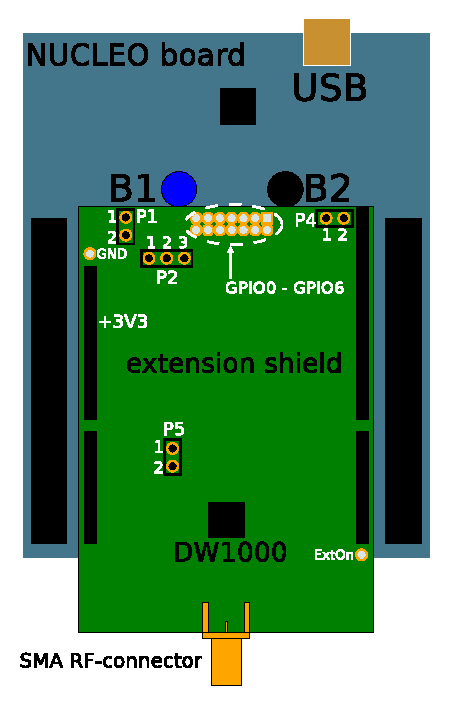
\includegraphics[width=2.5in]{Figures/Diagram11}%
		\label{fig:blockdiag}}
	\hfil
		\subfloat[Picture of the UWB extension shield stacked on top of the NUCLEO-L152RE board.]{\includegraphics[width=2.5in]{Figures/photo_small2}%
		\label{fig:photo}}
	\caption{The UWB extension shield stacked on top of the NUCLEO-L152RE board.}
	\label{fig:photodiag}
\end{figure*}
Figure~\ref{fig:photodiag} shows a block diagram (Figure~\ref{fig:blockdiag}) and a picture (Figure~\ref{fig:photo}) of the UWB platform without the optional boards. 
The NUCLEO-L152RE board can be extended through connectors that are compatible to the Arduino format~\cite{arduinowebsite}, as well as through the less flexible but more powerful MORPHO connectors. 
Additional hardware for programming the MCU is not necessary since an ST-Link programmer is already included. 
Another advantage is the flexibility to switch to different, compatible boards of the same product family (NUCLEO64), if necessary. 
If the application demands more computational power, more memory, or less energy consumption, the board can be exchanged with one that better fits the application requirements. 
Other extension shields can be stacked on top of the UWB board to complement the existing platform. 
This choice of hardware components sufficiently fulfilled our requirements from Table~\ref{tab:requirements}. 
The following detailed description explains our design decisions in the context of our requirements. 

\subsection{Fulfillment of the Requirements}
\label{subsec:implementingrequirements}

\vspace*{0.5em}
\noindent\textbf{IoT OS Support.} The Contiki operating system supports a variety of different processors and IoT platforms. 
The choice to use the STM32-based Nucleo board NUCLEO-L152RE brings multiple benefits, one of them being the support for both the STM32L152RE ARM-based Cortex-M3 CPU and the NUCLEO-L152RE platform. 
The driver for the DW1000 transceiver is not included in the official Contiki repository. 
However, an implementation exists~\cite{contikidw1000driver}. 

\vspace*{0.5em}
\noindent\textbf{Low-energy.} Of all hardware components in wireless sensor nodes the radio transceiver has the highest energy consumption. 
The chosen UWB transceiver DW1000 is no exception: in some operational modes, the average current consumption exceeds $150mA$. 
For small battery powered devices this is a problem. 
To reduce the DW1000's overall power consumption, an external DC-DC converter is used as proposed in~\cite[section 7.2]{dw1000ds}.
A crystal oscillator was used instead of a temperature-compensated crystal oscillator (TCXO) because of its higher energy efficiency. 

The Cortex-M3 CPU of the NUCLEO-L152RE is low-power and supports sleep as well as deep-sleep states~\cite{stm32ds}. 
The CPU has a current draw of $7.55mA@32MHz$ in active mode and $21.5\mu A$ in low-power sleep mode, which makes it suitable for battery-powered IoT devices. 

The DW1000 supports driving LEDs on four GPIO pins to indicate certain states of operation (transmitting, receiving, preamble received and start-of-frame delimiter received). 
This is useful for debugging, but it consumes more energy. 
Therefore the LEDs are included in the design but can be switched off by removing jumper P4. 
If there is no need for the LEDs on the platform, they can be left out on the board without affecting the functionality of the latter. 

The choice of using an external UWB antenna has an impact on energy efficiency as well as, because a higher antenna gain can increase the quality of a wireless communication link with the same energy budget. 

\vspace*{0.5em}
\noindent\textbf{Low-cost.} The NUCLEO-L152RE platform is a low-cost development platform that requires no additional programmer. %
The ST-Link software used to flash the micro-controller is open source and can be downloaded from~\cite{stlinkgithub}. % stm32flash in debian repo, stlink in community repo - archlinux
The firmware and the Contiki OS are open source too. %\unsure[inline]{not yet. has michael a plan to release his driver?}
Components like IMUs, IEEE 802.11 transceiver or other sensors can be added to the platform on demand and can be left out to reduce the overall cost of the platform. %\info{I can also mention the price of the wifi shield and the IMU shield}
The PCB manufacturing cost of 17.52EUR\footnote{We paid 175.20EUR for 10 pieces. The price heavily depends on the ordered quantity. The cost of ordering a single PCB is 126.42EUR.} accounts for the largest portion of the overall platform cost. 
The components per board sum up to 29.90EUR\footnote{Vendor www.mouser.com.} (see~\cite{berndrepo:prodtests} and Appendix~\ref{sec:bom} for details). 
A platform without the optional WiFi and MEMS boards would cost 47.42EUR. 
Including the WiFi board (18.79EUR) and the MEMS board (12.51EUR) the platform costs 78.72EUR. 

\vspace*{0.5em}
\noindent\textbf{Open source.} The software ST-Link is released under the BSD license. 
The Contiki OS source code is released under the Contiki open source license. 
The hardware design of the UWB extension shield was created using the Altium Designer software~\cite{altiumwebsite}. 
All design files and Gerber outputs are open-source as well. 
The UWB extension shield is designed to fit on the Arduino header, a common development platform that is also open source hardware.

\vspace*{0.5em}
\noindent\textbf{Individual power measurements.} The UWB extension shield was designed to allow power measurements. 
To measure the current consumption of the UWB extension shield, one can connect a current probe to jumper P1 (see Table~\ref{tab:jumpers} and Figure~\ref{fig:blockdiag}). 
In default mode, the jumper P1 must be shortened to connect the +3.3V supply pin from the Arduino header and the VCC plane from the UWB shield.

To measure the supply voltage of the extension shield, the voltage probe must be connected to the +3.3V supply pin and to the GND pin. 
To connect different types of probes, the GND test point next to the P1 jumper can be used.

\vspace*{0.5em}
\noindent\textbf{Multi-purpose solution.} The extension shield can be used in combination with different other MCU-boards. 
Nevertheless, it is possible to build sensor networks with wireless sensor nodes that all consist of the same hardware components. 
One is not forced to use specialized designs for different roles (like anchors or tags) in the network. 
If the application demands different hardware components in different nodes, the same UWB extension shield can be used in every sensor node. 
The SMA antenna connector simplifies the multi-purpose solution. 

\vspace*{0.5em}
\noindent\textbf{Exchangeable antenna} The SMA-RF connector allows experimenting with all antennas that have a female SMA connector. 
The user can choose an antenna design depending on the application. 
By using an RF switch one can use multiple antennas in the same design~\cite{Grosswindhager_Switchable_2017}.

\vspace*{0.5em}
\noindent\textbf{Expandability.} The decision to use the DW1000 on an extension shield was made to expand the hardware later on.
The platform's micro-controller can be changed without altering the UWB extension shield by stacking the extension shield on different MCU boards.
The chosen MCU board family (NUCLEO) offers two separate header formats for stacking - ST's own MORPHO header format and the widely used Arduino compatible header format. 
The advantage of the Arduino header connectors is that it is supported by a large community.
The UWB extension shield is designed to allow stacking of other extension shields.
Stacking two UWB extension shields is considered in the design and described in Section~\ref{subsec:pinusagejumpers}.
The P2 header (see Table~\ref{tab:jumpers} and Figure~\ref{fig:blockdiag}) was added to support two different SPI chip-select lines (SPI-CS).
This way, the same SPI bus can be used by another shield that is stacked on top of the UWB extension shield.
The header pins of the serial UART and I2C buses were left unused in the UWB extension shield, so that other extension shields can make use of them.
In particular the WiFi shield~\cite{wifiboard} and the sensor shield~\cite{memsboard} by ST are supported in combination with the UWB extension shield.

\vspace*{0.5em}
\noindent\textbf{Interface for data logging.} An interface for data logging can be stacked on top of the UWB extension shield. 
This can be a reliable second wireless interface like IEEE 802.11, or an offline mass storage to collect all test data for offline analysis. 
The WiFi shield X-NUCLEO-IDW04A1~\cite{wifiboard} supports both by providing access to an on-board micro SD card. 


%%%%%%%%%%%%%%%%%%%%%%%%%%%%%%%%%%%%%%%%%%%%%%%%%%%%%%%%%%%%%%%%%%%%%
\subsection{Pin Usage and Jumpers}
\label{subsec:pinusagejumpers}
Table~\ref{tab:headerconnectors} lists the names of the Arduino header connector pins. 
The communication buses SPI, I2C and UART are bold. 
The UART and I2C communication ports were left unused on the UWB extension shield so that the WiFi and MEMS boards can be used simultaneously. 
Three boards are listed in the table:
\begin{enumerate}
	\item NUCLEO-L152RE/STM32L152RE\\
	The labels of this board's connectors are CN6, CN8, CN5 and CN9. 
	In Figure~\ref{fig:3dview}, CN6 is connected to the UWB shield with the upper left, CN8 with the lower left connector, CN5 with the upper right and CN9  with the lower right.
	The pin names of the STM32L152RE are taken from the datasheet~\cite{stm32ds}.
	
	\item X-NUCLEO-IDW04A1\\
	The WiFi shield has multiple GPIO pins, but GPIO9, GPIO13, GPIO14 and GPIO15 cannot be used because they are reserved for the UWB shield's SPI pins.
	The X-NUCLEO-IDW04A1 is controlled using a UART bus interface.
	
	\item UWB Shield\\
	The DW1000 can only be controlled using the SPI bus.
	Therefore, using the SPI pins cannot be avoided on the UWB shield.
	The GPIOx pins of the UWB shield are optional.
	They are only connected to the CN9 header pins if the jumpers GPIO0 - GPIO6 are closed (see Table~\ref{tab:jumpers})
\end{enumerate}
The X-NUCLEO-IKS01A1 pins are not listed in Table~\ref{tab:headerconnectors}.
It is controlled using the I2C bus of CN5 and powered through CN6. %
Table~\ref{tab:jumpers} lists all the jumpers of the UWB shield.
\begin{table*}[t!]
	\centering
	\begin{tabular}{|c|c|l|l|}
		\hline
		\textbf{Jumper} & \textbf{Pin} & \textbf{Net Name} & \textbf{Description} \\ \hline\hline
		
		\multicolumn{1}{|c}{\multirow{2}{*}{P1} } &
		\multicolumn{1}{|c|}{P1-1} &
		+3V3 plane &
		positive voltage supply of UWB shield \\ \cline{2-4}
		
		\multicolumn{1}{|c}{} &
		\multicolumn{1}{|c|}{P1-2} & 
		+3V3 pin &
		positive voltage output of NUCLEO-L152RE header \\ \hline
		
		\multicolumn{1}{|c}{\multirow{3}{*}{P2} } &
		\multicolumn{1}{|c|}{P2-1} & 
		SPI-CS2 &
		alternative (2nd) SPI chip select \\ \cline{2-4}
		
		\multicolumn{1}{|c}{} &
		\multicolumn{1}{|c|}{P2-2} & 
		SPI-CS &
		SPI chip select of DW1000 \\ \cline{2-4}
		
		\multicolumn{1}{|c}{} &
		\multicolumn{1}{|c|}{P2-3} & 
		SPI-CS1 &
		default SPI chip select \\ \hline
		
		\multicolumn{1}{|c}{\multirow{2}{*}{P4} } &
		\multicolumn{1}{|c|}{P4-1} &
		LEDs cathodes &
		connected to the cathodes of all 4 LEDs \\ \cline{2-4}
		
		\multicolumn{1}{|c}{} &
		\multicolumn{1}{|c|}{P4-2} & 
		GND &
		connected to the ground plane of the UWB shield \\ \hline
		
		\multicolumn{1}{|c}{\multirow{2}{*}{P5} } &
		\multicolumn{1}{|c|}{P5-1} &
		+3V3 plane &
		connected to the positive voltage supply plane \\ \cline{2-4}
		
		\multicolumn{1}{|c}{} &
		\multicolumn{1}{|c|}{P5-2} & 
		DWM1000 VSS &
		connected to the supply pins of the optional DWM1000 \\ \hline
		
		\multicolumn{1}{|c}{\multirow{14}{*}{GPIO0-GPIO6} } &
		\multicolumn{1}{|c|}{GPIO0-1} &
		DW1000 pin 38 &
		connected to GPIO0 of DW1000 (LED\_RXOK)\\ \cline{2-4}
		
		\multicolumn{1}{|c}{} &
		\multicolumn{1}{|c|}{GPIO0-2} & 
		Pin 8 of CN9 &
		connected to pin number 8 of header CN9 \\ \cline{2-4}
		
		\multicolumn{1}{|c}{} &
		\multicolumn{1}{|c|}{GPIO1-1} & 
		DW1000 pin 37 &
		connected to GPIO1 of DW1000 (SFDLED) \\ \cline{2-4}
		
		\multicolumn{1}{|c}{} &
		\multicolumn{1}{|c|}{GPIO1-2} & 
		Pin 7 of CN9 &
		connected to pin number 7 of header CN9 \\ \cline{2-4}
		
		\multicolumn{1}{|c}{} &
		\multicolumn{1}{|c|}{GPIO2-1} & 
		DW1000 pin 36 &
		connected to GPIO2 of DW1000 (RXLED) \\ \cline{2-4}
		
		\multicolumn{1}{|c}{} &
		\multicolumn{1}{|c|}{GPIO2-2} & 
		Pin 6 of CN9 &
		connected to pin number 6 of header CN9 \\ \cline{2-4}
		
		\multicolumn{1}{|c}{} &
		\multicolumn{1}{|c|}{GPIO3-1} & 
		DW1000 pin 35 &
		connected to GPIO3 of DW1000 (TXLED) \\ \cline{2-4}
		
		\multicolumn{1}{|c}{} &
		\multicolumn{1}{|c|}{GPIO3-2} & 
		Pin 5 of CN9 &
		connected to pin number 5 of header CN9 \\ \cline{2-4}
		
		\multicolumn{1}{|c}{} &
		\multicolumn{1}{|c|}{GPIO4-1} & 
		DW1000 pin 34 &
		connected to GPIO4 of DW1000 (EXTPA) \\ \cline{2-4}
		
		\multicolumn{1}{|c}{} &
		\multicolumn{1}{|c|}{GPIO4-2} & 
		Pin 4 of CN9 &
		connected to pin number 4 of header CN9 \\ \cline{2-4}
		
		\multicolumn{1}{|c}{} &
		\multicolumn{1}{|c|}{GPIO5-1} & 
		DW1000 pin 33 &
		connected to GPIO5 of DW1000 (SPIPHA) \\ \cline{2-4}
		
		\multicolumn{1}{|c}{} &
		\multicolumn{1}{|c|}{GPIO5-2} & 
		Pin 3 of CN9 &
		connected to pin number 3 of header CN9 \\ \cline{2-4}
		
		\multicolumn{1}{|c}{} &
		\multicolumn{1}{|c|}{GPIO6-1} & 
		DW1000 pin 30 &
		connected to GPIO6 of DW1000 (SPIPOL) \\ \cline{2-4}
		
		\multicolumn{1}{|c}{} &
		\multicolumn{1}{|c|}{GPIO6-2} & 
		Pin 4 of CN9 &
		connected to pin number 3 of header CN8 \\ \hline
		
	\end{tabular}
	\caption{List of Jumpers and their purpose.}
	\label{tab:jumpers}
\end{table*}
\begin{table} [h!]
	\centering
	\begin{tabular}{|c|c|c|c|}\hline
	\textbf{Pin} & \textbf{STM32L152RE} & \textbf{WiFi Shield} & \textbf{UWB Shield} \\ \hline\hline
	  & \multicolumn{3}{c|}{CN6 (Power)} \\ \cline{2-4}
	1 & \multicolumn{3}{c|}{NC} \\ \cline{2-4}
	2 & \multicolumn{2}{c|}{3V3} & NC \\ \cline{2-4}
	3 & \multicolumn{2}{c|}{Reset Button} & NC \\ \cline{2-4}
	4 & \multicolumn{3}{c|}{3V3} \\ \cline{2-4}
	5 & \multicolumn{2}{c|}{5V} & NC \\ \cline{2-4}
	6 & \multicolumn{3}{c|}{GND} \\ \cline{2-4}
	7 & \multicolumn{3}{c|}{GND} \\ \cline{2-4}
	8 & \multicolumn{2}{c|}{VIN} & NC \\ \hline\hline
	  & \multicolumn{3}{c|}{CN8 (Analog)} \\ \cline{2-4}
	1 & PA0/ADC\_IN0 & NC & nRST \\ \cline{2-4}
	2 & PA1/ADC\_IN1 & NC & \textbf{CS2} \\ \cline{2-4}
	3 & PA4/ADC\_IN4 & NC & \textit{GPIO6} \\ \cline{2-4}
	4 & PB0/ADC\_IN8 & GPIO6 & SYNC/GPIO7 \\ \cline{2-4}
	5 & PC1/\textbf{SDA} & GPIO1 & NC \\ \cline{2-4}
	6 & PC0/\textbf{SCL} & \multicolumn{2}{c|}{NC} \\ \hline\hline
	  & \multicolumn{3}{c|}{CN5 (Digital)} \\ \cline{2-4}
	10 & PB8/\textbf{SCL} & GPIO5 & NC \\ \cline{2-4}
	9 & PB9/\textbf{SDA} & GPIO4 & NC \\ \cline{2-4}
	8 & \multicolumn{2}{c|}{AVDD} & NC \\ \cline{2-4}
	7 & \multicolumn{3}{c|}{GND} \\ \cline{2-4}
	6 & PA5/\textbf{SCK} & GPIO15 & \textbf{SCK} \\ \cline{2-4}
	5 & PA6/\textbf{MISO} & GPIO13 & \textbf{MISO} \\ \cline{2-4}
	4 & PA7/\textbf{MOSI} & GPIO14 & \textbf{MOSI} \\ \cline{2-4}
	3 & PB6/\textbf{CS} & NC & \textbf{CS1} \\ \cline{2-4}
	2 & PC7 & GPIO9 & \textbf{IRQ} \\ \cline{2-4}
	1 & PA9 & GPIO2 & WAKEUP \\ \hline\hline
	  & \multicolumn{3}{c|}{CN9 (Digital)} \\ \cline{2-4}
	8 & PA8 & WiFi RST & \textit{GPIO0} \\ \cline{2-4}
	7 & PB10 & PB10 & \textit{GPIO1} \\ \cline{2-4}
	6 & PB4 & PB4 & \textit{GPIO2} \\ \cline{2-4}
	5 & PB5 & PB5 & \textit{GPIO3} \\ \cline{2-4}
	4 & PB3 & NC & \textit{GPIO4} \\ \cline{2-4}
	3 & PA10 & GPIO11 & \textit{GPIO5} \\ \cline{2-4}
	2 & PA2/\textbf{UART\_TX} & GPIO11/\textbf{UART\_RX} & NC \\ \cline{2-4}
	1 & PA3/\textbf{UART\_RX} & \textbf{UART\_TX} & NC \\ \hline
	\end{tabular}
	\caption{Pin usage of header connectors.}
	\label{tab:headerconnectors}
\end{table}

\vspace*{0.5em}
\noindent\textbf{P1.} This jumper was added to the design to simplify current measurements.
The supply current of the UWB shield can be measured by connecting an ampere-meter to the pins P1-1 and P1-2.
P1 connects the voltage supply pin CN6-4 (see Table~\ref{tab:headerconnectors}) to the power plane (see Table~\ref{tab:stackup}) and must be closed for normal operation.

\vspace*{0.5em}
\noindent\textbf{P2.} The center pin P2-2 is connected to the DW1000's SPI chip select pin.
By closing P2-2 and P2-3 (on the right), the CN5-3 pin (see Table~\ref{tab:headerconnectors}) is used as the SPI chip select. 
This is the default use-case.
If P2-1 and P2-2 is closed instead, a second UWB shield (or any other shield that uses pin CN5-3 as SPI chip select) can be stacked onto the same NUCLEO-L152RE board.
Then the UWB shield can still communicate by using CN8-2 as SPI chip select.

\vspace*{0.5em}
\noindent\textbf{P4.} There are 4 LEDs that can be soldered on the UWB shield to indicate the communication state.
If GPIO0 - GPIO3 have to be used, the LEDs must be disconnected by opening P4.
This also helps saving energy.

\vspace*{0.5em}
\noindent\textbf{P5.} In case the optional DW\underline{M}1000 module is soldered on the UWB shield, P5 must be closed.
P5 connects the DWM1000's voltage supply to the power plane.
Both the DW1000 and the DWM1000 can be used at the same time. 
For simultaneous use, the DW1000 must be connected to CS1 by closing P2-2 and P2-3. 
The DWM1000's SPI-CS is connected to CS2 (CN8-2).
If there is no DWM1000 soldered on the UWB shield, the state of P5 is irrelevant.

\vspace*{0.5em}
\noindent\textbf{GPIO0 - GPIO6.} There are 8 GPIOs on the DW1000 that can be controlled by the firmware. 
GPIO7 is connected to CN8-4.
GPIO0 to GPIO6 are accessible to the user in two ways. 
One way is to attach measurement probes to the test points on the edge of the board. 
The other way would be to solder a pin header onto these test points or shorten them using solder bridges (in Figure~\ref{fig:photo} the pin header is soldered onto the board). 
Then the GPIOs are accessible to the NUCLEO-L152RE board via its CN9 header pins as well. 
Closing these jumpers is optional. 
By closing the GPIOx jumpers, the DW1000's GPIO0 - GPIO5 pins are connected to the CN9-8 - CN9-3 pins and GPIO6 is connected to CN8-3 (see Table~\ref{tab:headerconnectors}).


%%%%%%%%%%%%%%%%%%%%%%%%%%%%%%%%%%%%%%%%%%%%%%%%%%%%%%%%%%%%%%%%%%%%%
\subsection{Production Specifics of the UWB Extension Shield}
\label{subsec:hwdesignuwbshield}
Figure~\ref{fig:altiumscreenshots} shows our design of the UWB extension shield with Figure~\ref{fig:3dview} showing the top view.
In Figure~\ref{fig:2dview} the copper elements of the top layer are colored in red and the copper elements of the bottom layer are colored in blue. 
\begin{figure*}[t!]
	\centering
		\subfloat[Top view of UWB extension shield.]{\includegraphics[width=2.5in]{Figures/board}%
		\label{fig:3dview}}
	\hfil
		\subfloat[PCB Designer view of UWB extension shield.]{\includegraphics[width=2.5in]{Figures/pcbdesign}%
		\label{fig:2dview}}
	\caption{UWB extension shield design.}
	\label{fig:altiumscreenshots}
\end{figure*}

Decawave provides its own design guide for integrating the DW1000 in a hardware design~\cite{dw1000hwdesignguide}.
This hardware design guide and Decawave's own reference design for the DW1000 (the EVK1000 evaluation platform~\cite{evk1000um}) were kept in mind for the UWB extension shield design.

As discussed earlier, the manufacturing of the PCB is the main cost factor. 
The following parameters affect the PCB cost and should hence be considered:
\begin{itemize}
	\item Size (area);
	\item Number of Layers;
	\item Quantity;
	\item Surface finish;
	\item Track width;
	\item Via diameter;
	\item Material of dielectric;
	\item Color of solder stop;
	\item (optional) Solder stencil\footnote{When soldering in a reflow-oven, a stencil is helpful to deposit the soldering paste onto the SMT pads.}.
\end{itemize}
Although the cost should be minimized, we decided to make the following trade-offs to ensure a high quality design. 

\vspace*{0.5em}
\noindent\textbf{Track width.} A smaller track width leads to higher production costs. 
The minimum track width of the PCB design is limited by the pad width of the DW1000, which is $200\mu m$.

\vspace*{0.5em}
\noindent\textbf{4-Layer layout.} The choice of a 4-layer layout instead of a cheaper 2-layer layout had two reasons: (i) to decrease the width of the RF transmission lines (see Section~\ref{subsec:txlinedesign}) and (ii) to simplify the uniform power supply while placing the components close to each other.
The placement of the decoupling capacitors is crucial to the performance of the DW1000. 
A 4-layer layout allows to place them very close to the DW1000's pins.
The second and third layer in the 4-layer layout are assigned to be a VCC plane (positive voltage power supply) and a GND plane (negative voltage power supply), respectively. 
That way, these two nets are accessible through vias anywhere on the PCB. 
Section~\ref{subsec:layerstackup} gives detailed description of the layer stackup.

\vspace*{0.5em}
\noindent\textbf{Board size.} A larger area increases the costs of the extension shield. 
The minimum width of the PCB results from using the Arduino header connector, which is $50.26mm$.
To have a safe distance between the SMA connector, the RF transmission lines and the underlying NUCLEO-L152RE board, the length of the board is $60mm$.
That is $10.74mm$ longer than the minimum length forced by the Arduino header.

\vspace*{0.5em}
\noindent\textbf{Electroless Nickel Immersion Gold (ENIG).} This type of surface plating is more expensive compared to other techniques.
One of its advantages is the constant surface planarity. 
The surface thickness must be considered when calculating the dimensions of the RF transmission lines. 
A deviation of the surface thickness would lead to a incorrect width of the transmission lines.

\vspace*{0.5em}
\noindent\textbf{Manufacturer.} We chose the manufacturer Multi-CB~\cite{mcbwebsite} to produce our PCBs.
Though the layer stackup recommended by Decawave~\cite[Figure 5]{dw1000hwdesignguide} was not offered, an individual layer stackup was possible. 
Detailed information about thickness and material of each layer was available and was considered in the calculation of the transmission line width.
The layer stackup is described in detail in Section~\ref{subsec:layerstackup}.

\vspace*{0.5em}
\noindent\textbf{Components placement.} Possible positions for the antenna port were the top or the bottom edge of the PCB. 
The bottom edge was chosen to increase the UWB antenna's distance to all other electronic components. 
Placing the DW1000 in the middle of the board would allow good access to all 48 of its pins. 
To keep the length of the transmission lines as short as possible (and therefore the chance of impedance deviations), the DW1000 was instead, placed closer to the bottom edge (see Section~\ref{subsec:txlinedesign} for details).
One design aspect that was not obvious before we soldered the UWB shields was the correct alignment of the stencil.
The pads of R7 (close to P2) were very helpful to align the stencil on the PCB. 

%%%%%%%%%%%%%%%%%%%%%%%%%%%%%%%%%%%%%%%%%%%%%%%%%%%%%%%%%%%%%%%%%%%%%
\subsection{Custom SMA Footprint Library}
\label{subsec:smafootprint}

The SMA connector must not be through-hole mounted, but should be edge-mounted. 
A through-hole mounted connector would add an unwanted stub to the transmission line. 
In our design the footprint of the SMA connector is customized to avoid impedance discontinuities. 
The pad width of the center pin that carries the signal is matched to have the same width as the transmission line. 
Furthermore, the pad length of the signal pin was increased until the edge of the PCB so that there is no gap between the transmission line and the PCB edge.

%%%%%%%%%%%%%%%%%%%%%%%%%%%%%%%%%%%%%%%%%%%%%%%%%%%%%%%%%%%%%%%%%%%%%
\subsection{PCB Layer Stackup}
\label{subsec:layerstackup}
\begin{table*}[h!]
	\centering
	\begin{tabular}{cc|l|r|}
	\multicolumn{1}{c}{} & \multicolumn{1}{c}{Name} & \multicolumn{1}{c}{Material} & \multicolumn{1}{c}{Thickness [$\mu m$]} \\ \cline{2-4}
\multicolumn{1}{c}{\multirow{11}{*}{\includegraphics[height=12em]{Figures/layerstackup1}}} 
						& \multicolumn{1}{l|}{Top Overlay }	& Ink			&     \\ \cline{2-4}
\multicolumn{1}{c}{}	& \multicolumn{1}{l|}{	Top Solder}  	& Solder-Stop	&  10 \\ \cline{2-4}
\multicolumn{1}{c}{}	& \multicolumn{1}{l|}{	Component Side}	& Copper		&  35 \\ \cline{2-4}
\multicolumn{1}{c}{}	& \multicolumn{1}{l|}{	Dielectric }		& 2 x Prepreg 7628 & 180+180 \\ \cline{2-4}
\multicolumn{1}{c}{}	& \multicolumn{1}{l|}{	Ground Plane }	& Copper		&  18 \\ \cline{2-4}
\multicolumn{1}{c}{}	& \multicolumn{1}{l|}{	Dielectric 	}	& FR-4 Core		& 700 \\ \cline{2-4}
\multicolumn{1}{c}{}	& \multicolumn{1}{l|}{	Power Plane }	& Copper		&  18 \\ \cline{2-4}
\multicolumn{1}{c}{}	& \multicolumn{1}{l|}{	Dielectric 	}	& 2 x Prepreg 7628 & 180+180 \\ \cline{2-4}
\multicolumn{1}{c}{}	& \multicolumn{1}{l|}{	Solder Side }	& Copper		&  35 \\ \cline{2-4}
\multicolumn{1}{c}{}	& \multicolumn{1}{l|}{	Bottom Solder }	& Solder-Stop	&  10 \\ \cline{2-4}
\multicolumn{1}{c}{}	& \multicolumn{1}{l|}{	Bottom Overlay }	& Ink			&     \\ \cline{2-4}
	\end{tabular}
	\caption{Thickness and Material of the 4-Layer PCB Stackup~\cite{altiumwebsite}.}
	\label{tab:stackup}
\end{table*}
Table~\ref{tab:stackup} shows the layer names, the chosen FR4 types and their thickness. 
In total, the PCB has a thickness of $1\,526\mu m$. 
A symmetric layer stackup was demanded by the manufacturer. 
Especially the dielectric between the component side, where the transmission lines are located and the underlying GND plane is of interest.
Using two layers of Prepreg 7628 with a combined thickness of $360\mu m$ came closest to the recommendation in~\cite{dw1000hwdesignguide}. 
The manufacturer Multi-CB also provided information about the Prepreg that will be used for production.
In our case, this was the DE104 by Isola Group~\cite{fr4datasheet}.
According to the DE104 datasheet, the \textbf{permittivity} at $5GHz$ is $\epsilon_r = 4.32$. 
These two values - the thickness and the permittivity - will affect the dimension of the transmission lines (see Section~\ref{subsec:txlinedesign}).

%%%%%%%%%%%%%%%%%%%%%%%%%%%%%%%%%%%%%%%%%%%%%%%%%%%%%%%%%%%%%%%%%%%%%
\subsection{Placing Decoupling Capacitors}
\label{subsec:placingcaps}
The decoupling networks must fulfill two purposes.
First, they must filter noise and other high frequency signals. 
Second, they act as energy buffers. 
To effectively filter high frequency signals, the capacitance should be small and the component must be placed close to the signal source.

The current path must be considered when placing the capacitors.
A decoupling is only possible if the pads of the capacitor are positioned between the power source and the DW1000 pad.
Figure~\ref{fig:decap} shows capacitor C22 to illustrate the correct placement of decoupling capacitors.

The power amplifier pins VDDPA1 and VDDPA2 of the DW1000 are decoupled by a network of 7 capacitors to avoid noise propagation to other parts of the board. 
See~\cite[chapter 6.3]{dw1000hwdesignguide} for a detailed explanation on how to place them.
\begin{figure}[h!]
	\centering
	\includegraphics[width=0.3\textwidth]{Figures/decap}
	\caption{Correct decoupling capacitor placement.}
	\label{fig:decap}
\end{figure}

%%%%%%%%%%%%%%%%%%%%%%%%%%%%%%%%%%%%%%%%%%%%%%%%%%%%%%%%%%%%%%%%%%%%%
\subsection{Transmission Line Design}
\label{subsec:txlinedesign}
Designing the transmission lines can be challenging, because even small miscalculations could cause problems. 
We included a backup solution in our PCB design in case of unforeseen problems, which is described in Section~\ref{subsec:dwm1000footprint}.

Figure~\ref{fig:txlines} shows the transmission lines on the UWB shield.
The differential transmission lines connecting the DW1000's RF\_P and RF\_N pins to the capacitors C9 and C10 must have $100\Omega$.
The second differential pair connects the capacitors to the UWB Balun and must have $50\Omega$.
Finally a $50\Omega$ single-ended transmission line connects the Balun to the SMA signal pin.
\begin{figure}%[h!]
	\centering
	\includegraphics[width=2.5in]{Figures/txlines}
	\caption{RF transmission lines.}
	\label{fig:txlines}
\end{figure}
There is a rule of thumb in RF design saying that a connection in a network must be treated as a transmission line if it is longer than $\lambda / 10$.
Assuming the highest frequency on these transmission lines is 10GHz, this would lead to a length of $3mm$ to be considered.
\begin{equation}
\label{eq:lambda10}
\frac{\lambda}{10} = \frac{1}{10} \cdot \frac{speed\;of\;light}{frequency} = \frac{1}{10} \cdot \frac{299\,792\,458 \frac{m}{s}}{10\cdot 10^9 \frac{1}{s}} = 3mm
\end{equation}
For the same reason, the components on the UWB shield have the housing size of \textbf{0402}\footnote{0402 is a standard package size for SMT components. The dimensions are 1.0mm x 0.5mm.}. 
A bigger housing would require to treat that component like a transmission line. 
According to~\eqref{eq:lambda10}, the transmission lines can be treated as normal connections as long as they are shorter than $3mm$.
This was taken into account when designing the PCB. 
In the final design, the transmission lines seen in Figure~\ref{fig:txlines} had the lengths listed in Table~\ref{tab:lengthstxlines}.
\begin{table}[t!]
	\centering
	\begin{tabular}{lr}
	\multicolumn{1}{c}{Net} & \multicolumn{1}{c}{Length in $mm$} \\ \hline
	$100 \Omega$ differential & 1.18 \\
	$50 \Omega$ differential & 0.35 \\
	$50 \Omega$ single-ended & \textbf{5.4}
	\end{tabular}
	\caption{Lengths of (potential) transmission lines.}
	\label{tab:lengthstxlines}
\end{table}
Line impedance matching by calculating the correct width was neglected for connections shorter than $3mm$.
So only the connection from the Balun to the SMA connector was treated as a transmission line.
The model to calculate the correct width of the $50 \Omega$ single-ended transmission line is illustrated in Figure~\ref{fig:pcbcalc}.
$T$ is the thickness of the copper on the component side.
As mentioned before in Section~\ref{subsec:hwdesignuwbshield}, there are fabrication methods that guarantee an almost constant thickness.
$H$ is the thickness of the dielectric. 
In this case, it is a $360\mu m$ thick FR-4 (see Table~\ref{tab:stackup}) having an $\epsilon_r = 4.32$ at $5 \; GHz$~\cite{fr4datasheet}.
Another rule of thumb says that the space between the shielding GND planes and the transmission line should be twice the transmission line's width.
%Hence, the distance of the co-planar GND planes to the transmission lines is $S = 2\cdot 0.7mm = 1.4mm$.
\begin{figure}%[h]
	\centering
	\includegraphics[width=0.3\textwidth]{Figures/pcbcalc}
	\caption{Scheme for transmission lines with co-planar wave guide and ground plane.}
	\label{fig:pcbcalc}
\end{figure}
There are several vias added to the GND planes on both sides of the $50\Omega$ transmission line to improve the shielding of the transmission line.

The area around the transmission lines must be free from solder stop and printed text, because these layers are not taken into account when calculating the trace width of the transmission line.

\vspace*{0.5em}
\noindent\textbf{Transmission line calculator tools.} The Altium Designer software includes some helpful tools to design transmission lines~\cite{altiumwebsite}.
By providing the layer stackup (Table~\ref{tab:stackup}) and defining the desired line impedance, Altium automatically calculates the line width.
There are several other tools available to calculate the width of a transmission line.
Their results are listed in Table~\ref{tab:txlinecalculations}.
Even though the results are different, their deviation is still within the manufacturing tolerances.
We took the value calculated by Altium Designer for our design.
\begin{table}[h!]
	\centering
	\begin{tabular}{lr}
	\multicolumn{1}{c}{Tool} & \multicolumn{1}{c}{Result for $W$ in $\mu m$} \\ \hline
	Altium 17~\cite{altiumwebsite} & \textbf{700} \\
	Multi-CB Online Tool~\cite{mcbwebsite} & 636 \\
	PCB Calculator~\cite{kicadwebsite} & 710 \\
	NI AWR TX Line~\cite{nitxlinewebsite} & 672 \\
	Saturn PCB~\cite{saturnwebsite} & 740 \\
	\end{tabular}
	\caption{Results for $W$ calculated by different tools.}
	\label{tab:txlinecalculations}
\end{table}

%%%%%%%%%%%%%%%%%%%%%%%%%%%%%%%%%%%%%%%%%%%%%%%%%%%%%%%%%%%%%%%%%%%%%
\subsection{DWM1000 Footprint}
\label{subsec:dwm1000footprint}
The UWB extension shield design includes a backup solution by soldering a DWM1000 module~\cite{dwm1000ds}.
The footprint was added to the PCB layout in case the RF transmission line design of the DW1000 is faulty or shows insufficient performance.
That way the PCBs would still be of use. 
Another advantage is that the DWM1000 and the DW1000 can be used in the same design.
This can be useful for comparing the performance of the DWM1000's omni-directional UWB antenna with individual designs.
Listening on different RF channels at the same time is also possible.

%%%%%%%%%%%%%%%%%%%%%%%%%%%%%%%%%%%%%%%%%%%%%%%%%%%%%%%%%%%%%%%%%%%%%
\subsection{Crystal}
\label{subsec:crystaldesign}
The DW1000 uses a 38.4 MHz quartz crystal to synthesize the frequencies for RF TX, RF RX and all digital blocks. 
Since ranging and localization applications rely on precise time measurements, the accuracy of the crystal is crucial for their performance.
Ambient temperature changes have a strong impact on the clock drift of the quartz crystal.
This can be omitted by using a temperature-compensated crystal instead of a simple one.
In Section~\ref{subsec:implementingrequirements} it was mentioned that we are not using a TCXO in favor of a lower energy consumption. 
A low frequency tolerance and frequency drift of $\pm 10ppm$ are recommended in the DW1000 datasheet alongside with three crystals by different manufacturers~\cite{dw1000ds}.
Because none of these three recommended crystals were available for purchase at design time, we decided to use Epson's TSX-3225 in our design~\cite{crystalds}.
The TSX-3225 is a 10ppm crystal oscillator with the same specifications as the RSX10 used by the EVK1000~\cite{evk1000um}.

The DW1000 offers a crystal calibration mechanism to compensate for the initial frequency offset.
The procedure to trim the crystal is described in detail in Appendix~\ref{subsubsec:crystaltrim}.

In the PCB layout, the crystal must be placed as close as possible to the XTAL1 and XTAL2 pins.
To avoid too much noise interference by the DC-DC converter, the DC-DC converter was placed on the opposite side of the DW1000, as recommended in the hardware design reference guide~\cite{dw1000hwdesignguide}.

% one can use the crystal trim to compensate for temperature changes. But the temperature monitor can only monitor the DW1000 temperature, not the crystal temperature.

%%%%%%%%%%%%%%%%%%%%%%%%%%%%%%%%%%%%%%%%%%%%%%%%%%%%%%%%%%%%%%%%%%%%%%
%%%%%%%%%%%%%%%%%%%%%%%%%%%%%%%%%%%%%%%%%%%%%%%%%%%%%%%%%%%%%%%%%%%%%%
%%%%%%%%%%%%%%%%%%%%%%%%%%%%%%%%%%%%%%%%%%%%%%%%%%%%%%%%%%%%%%%%%%%%%%
\section{Limitations}
\label{sec:limitations}

\subsection{Optional DWM1000}
\label{subsec:optionaldw1000}
If the optional DWM1000 module is soldered on the board in addition to the DW1000 transceiver, the SPI communication can be unreliable if the DWM1000 is not powered.
The voltage supply of the DWM1000 module can be assured by closing jumper P5. 
It connects the voltage supply pins of the DWM1000 to the 3V3 net of the extension shield. While the DWM1000 is supplied, its MISO, MOSI and SCK pins have a high impedance of 50 to 90 $k\Omega$. 
If the module is not supplied, the pins are floating and can unintentionally pull down the voltage and, therefore, disturb the SPI communication to the DW1000.
Figure~\ref{fig:badspiclk} shows the clock signal if the DWM1000 is present and P5 is open, while Figure~\ref{fig:goodspiclk} shows the same signal with P5 closed.
In both figures, measured using a digital storage oscilloscope, the upper and lower threshold for detecting if the input signal state is HIGH or LOW are sketched.
In Figure~\ref{fig:badspiclk} the SPI clock signal never exceeds the upper threshold.
Because the SPI clock state as detected by the DW1000 stays at LOW, the communication to the DW1000 is impossible.
\begin{figure}[h!]
	\centering
	\includegraphics[width=0.5\textwidth]{Figures/sck_bare_init}
	\caption{Oscilloscope measurement of the distorted SPI clock signal.}
	\label{fig:badspiclk}
\end{figure}
\begin{figure}[h!]
	\centering
	\includegraphics[width=0.5\textwidth]{Figures/sck_contiki_txrx}
	\caption{Oscilloscope measurement of the valid SPI clock signal.}
	\label{fig:goodspiclk}
\end{figure}

\subsection{Optional DC/DC Converter}
The component \textbf{U2} on the board is the DC-DC step down converter. 
By supplying certain pins of the DW1000 with 1.8V instead of 3.3V, the transceiver consumes less energy. 
However, the footprint of this component is mirrored unintentionally in the design and hence the DC-DC converter cannot be used. 
The pads U2-2 and U2-4 must be shortened with a piece of wire to supply all DW1000 pins as shown in Figure~\ref{fig:dcdc}.
\begin{figure}%[h!]
	\centering
	\includegraphics[width=0.2\textwidth]{Figures/dcdc}
	\caption{Work-around for faulty DC-DC footprint.}
	\label{fig:dcdc}
\end{figure}
In a future design, the footprint should be mirrored to use the DC-DC converter for saving energy.

\subsection{Marking}
On the top layer of the board, the label for the SYNC pin beneath GPIO6 is missing.
The next design should include that label.
All texts should be written in the same font size as well (the CN6 pin labels have a larger font size than the others).

\subsection{TCXO Footprint}
In the next design, it should be possible to choose between a TCXO and a normal quartz crystal.
The TCXO usually has 6 connectors, because it must be connected to a low noise power source.
If a TCXO is used, an additional low-dropout regulator (LDO) must be added.


%%%%%%%%%%%%%%%%%%%%%%%%%%%%%%%%%%%%%%%%%%%%%%%%%%%%%%%%%%%%%%%%%%%%%
%%%%%%%%%%%%%%%%%%%%%%%%%%%%%%%%%%%%%%%%%%%%%%%%%%%%%%%%%%%%%%%%%%%%%
%%%%%%%%%%%%%%%%%%%%%%%%%%%%%%%%%%%%%%%%%%%%%%%%%%%%%%%%%%%%%%%%%%%%%
\section{Evaluation and Calibration of the UWB Platform}
\label{sec:testingandcalibrating}
After soldering the UWB extension shields in a re-flow oven, the production tests for DW1000 based circuits were performed~\cite{prodtest}.
A description how to execute these tests on our UWB platform can be found in Appendix~\ref{sec:prodtests}.

For voltage- and current measurements the Fluke 87-V Digital Multimeter was used.
Transmit power and crystal frequency were calibrated using the Rohde-Schwarz FSQ26 Spectrum Analyzer.

%%%%%%%%%%%%%%%%%%%%%%%%%%%%%%%%%%%%%%%%%%%%%%%%%%%%%%%%%%%%%%%%%%%%%
\subsection{Operational Tests}
\label{subsec:optests}
\begin{table}[h!]
	\centering
	\begin{tabular}{|c|c|}
		\hline
		\textbf{Current after 10s} & \textbf{Voltage} \\ \hline
		[mA] & [mV] \\ \hline\hline
		18.88 & 3270 \\
		\hline		
	\end{tabular}
	\vspace{1.5mm}
	\caption{Idle current measurement.}
	\label{tab:resultsidlecurrent}
\end{table}
The current consumption of the board in idle mode was within the expected range (see Table~\ref{tab:resultsidlecurrent}).
The SPI test executed successfully.
So did the GPIO strobe test, the RSTn test, the EXTON test and the WAKEUP test.
The results of the maximum current consumption are listed in Table~\ref{tab:resultmaxcurrent}.
\begin{table}[h!]
	\centering
	\begin{tabular}{|c|c|}
		\hline
		\textbf{Maximum current consumption} & \textbf{Voltage} \\ \hline
		[mA] & [mV] \\ \hline\hline
		220 & 3268 \\
		\hline
	\end{tabular}
	\vspace{1.5mm}
	\caption{Maximum current measurement.}
	\label{tab:resultmaxcurrent}
\end{table}
The operational tests showed a maximum current consumption that was much higher than expected (see Table~\ref{tab:resultmaxcurrent}).
The reason for that is not clear yet.
A design flaw in the UWB shield is not suspected, because this can be measured using the DWM1000 too.


\subsection{Transmitter Calibration}
\label{subsec:txcalibration}

\vspace*{0.5em}
\noindent\textbf{Crystal calibration.} The remaining frequency offset was the smallest at the crystal trim value \texttt{0x16}. 
On channel 5, the remaining offset was $0.008974MHz$ and on channel 4 the spectrum analyzer showed a remaining offset of $0.0MHz$.
Captures of the measurements for channel 5 are shown in Figure~\ref{fig:resxtaltrim5} and for channel 4 in Figure~\ref{fig:resxtaltrim4}.
\begin{figure}
	\centering
	\includegraphics[width=0.55\textwidth]{Figures/07_XTALTRIM}
	\caption{Result of crystal calibration on channel 5. The marker 1 shows that the peak is at a frequency of $6.489608974 \; GHz$.}
	\label{fig:resxtaltrim5}
\end{figure}
\begin{figure}
	\centering
	\includegraphics[width=0.55\textwidth]{Figures/07_XTALTRIM_CH4}
	\caption{Result of crystal calibration on channel 4.}
	\label{fig:resxtaltrim4}
\end{figure}
In every subsequent test this crystal trim value was configured.

\begin{table*}[h!]
	\centering
	\begin{tabular}{|c|c|c|c|c|c|r|r|r|}
	\hline
	\textbf{Test number} & \textbf{Channel} & \textbf{Frequency} & \textbf{Bandwidth} & \textbf{PRF} & \textbf{Code} & \textbf{Coarse Gain (reference)} & \textbf{Fine Gain (reference)} & \textbf{PGDELAY (reference)}\\ \hline
	& & [MHz] & [MHz] & [MHz] & & dB & dB & \\\hline\hline
	 1 & 1 & 3494.4 & 499.2  & 16 & 1 & 9 (+0)& 10.5 (+0)& \texttt{0xC9} (+0) \\ \hline
  	 2 & 1 & 3494.4 & 499.2  & 64 & 9 & 9 (+0)& 3.5 (+0)& \texttt{0xD0} (+7) \\ \hline
	 3 & 2 & 3993.6 & 499.2  & 16 & 3 & 9 (+0)& 9.5 (-1) & \texttt{0xD4} (+15) \\ \hline
	 4 & 2 & 3993.6 & 499.2  & 64 & 9 & 9 (+0)& 3.5 (+0)& \texttt{0xD4} (+15) \\ \hline
	 5 & 3 & 4492.8 & 499.2  & 16 & 5 & 9 (+0)& 9.0 (+1.5)& \texttt{0xD1} (+12) \\ \hline
	 6 & 3 & 4492.8 & 499.2  & 64 & 9 & 6 (+0)& 6.0 (-0.5)& \texttt{0xD1} (+12)\\ \hline
	 7 & 4 & 3993.6 & 1331.2 & 16 & 7 &\textbf{15 (+3)}&\textbf{12.0 (+3.5)}& \texttt{0x95} (+0)\\ \hline
	 8 & 4 & 3993.6 & 1331.2 & 64 & 9 & 6 (+0)&11.5 (-2.5)& \texttt{0x95} (+0)\\ \hline
	 9 & 5 & 6489.6 & 499.2  & 16 & 3 &12 (+0)& 3.0 (+1)& \textbf{\texttt{0xD2} (+18)}\\ \hline
	10 & 5 & 6489.6 & 499.2  & 64 & 9 & 6 (+0)& 1.5 (-1)& \textbf{\texttt{0xD2} (+18)}\\ \hline
	11 & 7 & 6489.6 & 1081.6 & 16 & 7 & 6 (+0)&13.0 (+4)&  \texttt{0x93} (+0)\\ \hline
	12 & 7 & 6489.6 & 1081.6 & 64 &17 & 0 (+0)&12.0 (+3.5)& \texttt{0x93} (+0)\\ \hline
	\end{tabular}
	\caption{Measurements of Transmit Power. $+3$ means we had to increase the reference value by 3, $-1$ means we had to decrease the reference value by 1.
$+0$ indicates where the reference value was left unchanged.}
	\label{tab:resulttxpowermeasurements}
\end{table*}
\vspace*{0.5em}
\noindent\textbf{Transmit power calibration.} The attenuation of the SMA cable was about $1dB$ across all tested frequencies.
We configured the spectrum analyzer offset to take that attenuation into account, so we did not need to subtract it later as described in Appendix~\ref{subsubsec:transmitpowercalibration}.
Along with the transmit power, we adjusted the bandwidth as well.
The bandwidth can be adjusted by changing the UWB pulse width.
The column for the pulse generator delay (PGDELAY) lists the calibrated values for register \texttt{2A:0B}.
By increasing the pulse generator delay, the pulse width (and the transmit power) increases and the bandwidth decreases.
If this value is decreased, the bandwidth increases (and the transmit power decreases).
The measurement results are listed in Table~\ref{tab:resulttxpowermeasurements}.
The numbers in brackets indicate the difference to the reference values from the DW1000 user manual~\cite{dw1000um}.
Figure~\ref{fig:txpowermeasurements123} and Figure~\ref{fig:txpowermeasurements457} show the spectrum for all channels and pulse repetition frequencies (PRF).
Outside the band, the transmit power has to be $10dB$ below the maximum limit of $-41.3 \; dBm/MHz$.

\begin{figure}[b!]
	\centering
	\includegraphics[width=0.5\textwidth]{Figures/histogram}
	\caption{Histogram of ranging measurements.}
	\label{fig:antennadelayranging}
\end{figure}

\begin{figure*}%[h!]
	\centering
		\subfloat[Channel 1 at 16MHz PRF]{\includegraphics[width=0.4\textwidth]{Figures/TEST1_CH1_16M}%
		\label{fig:TEST1_CH1_16M}}
	\hfil
		\subfloat[Channel 1 at 64MHz PRF]{\includegraphics[width=0.4\textwidth]{Figures/TEST2_CH1_64M}%
		\label{fig:TEST2_CH1_64M}}
		\\
	\subfloat[Channel 2 at 16MHz PRF]{\includegraphics[width=0.4\textwidth]{Figures/TEST3_CH2_16M}%
		\label{fig:TEST3_CH2_16M}}
	\hfil
		\subfloat[Channel 2 at 64MHz PRF]{\includegraphics[width=0.4\textwidth]{Figures/TEST4_CH2_64M}%
		\label{fig:TEST4_CH2_64M}}
		\\
	\subfloat[Channel 3 at 16MHz PRF]{\includegraphics[width=0.4\textwidth]{Figures/TEST5_CH3_16M}%
		\label{fig:TEST5_CH3_16M}}
	\hfil
		\subfloat[Channel 3 at 64MHz PRF]{\includegraphics[width=0.4\textwidth]{Figures/TEST6_CH3_64M}%
		\label{fig:TEST6_CH3_64M}}
	\caption{Transmit Power and Bandwidth on Channels 1, 2, and 3 for 16 and 64MHz PRF, respectively.}
	\label{fig:txpowermeasurements123}
\end{figure*}

\begin{figure*}%[h!]
	\centering
		\subfloat[Channel 4 at 16MHz PRF]{\includegraphics[width=0.4\textwidth]{Figures/TEST7_CH4_16M}%
		\label{fig:TEST7_CH4_16M}}
	\hfil
		\subfloat[Channel 4 at 64MHz PRF]{\includegraphics[width=0.4\textwidth]{Figures/TEST8_CH4_64M}%
		\label{fig:TEST8_CH4_64M}}
		\\
	\subfloat[Channel 5 at 16MHz PRF]{\includegraphics[width=0.4\textwidth]{Figures/TEST9_CH5_16M}%
		\label{fig:TEST9_CH5_16M}}
	\hfil
		\subfloat[Channel 5 at 64MHz PRF]{\includegraphics[width=0.4\textwidth]{Figures/TEST10_CH5_64M}%
		\label{fig:TEST10_CH5_64M}}
		\\
	\subfloat[Channel 7 at 16MHz PRF]{\includegraphics[width=0.4\textwidth]{Figures/TEST11_CH7_16M}%
		\label{fig:TEST11_CH7_16M}}
	\hfil
		\subfloat[Channel 7 at 64MHz PRF]{\includegraphics[width=0.4\textwidth]{Figures/TEST12_CH7_64M}%
		\label{fig:TEST12_CH7_64M}}
	\caption{Transmit Power and Bandwidth on Channels 4, 5, and 7 for 16 and 64MHz PRF, respectively.}
	\label{fig:txpowermeasurements457}
\end{figure*}



\vspace*{0.5em}
\noindent\textbf{Antenna delay calibration.} After the crystal oscillator and the transmit power and bandwidth, the antenna delay can be calibrated.
The DW1000 supports a special transmit mode for time-of-flight measurements.
In this mode, the timestamps of received and transmitted packets are saved to a register.
The timestamp is internally corrected by taking the antenna delay into account, when reading the timestamp from the register.
The antenna delay is the time duration between a frame being processed digitally and the corresponding RF signal passing the antenna.
For reception and transmission the antenna delay is different.
The ranging accuracy can be increased from 30cm to 4.5cm by calibrating the antenna delay~\cite{dw1000antdelcal}.
A description of the test procedure can be found in Section~\ref{subsec:antennadelay}.
Figure~\ref{fig:antennadelayranging} shows the histogram of 10000 ranging measurements.

The test boards were connected using a 100cm long coaxial cable\footnote{Harbour Industries M17/152-00001 MIL-DTL-17, tested for a maximum frequency of 12.4 GHz.}. 
This gives a combined antenna delay of:
\begin{equation}
\label{eq:antdelcalc}
Delay_{TX,RX} = \frac{155.29m - 1.0m}{299702547\frac{m}{s}} = 514.81ns
\end{equation}
The antenna delay for transmitted frames is then given by~\eqref{eq:antdelcalctx1} and by~\eqref{eq:antdelcalcrx1} for received frames (see Appendix~\ref{subsec:antennadelay}).
Processing received frames takes slightly longer than transmitting frames.
The combined delay is apportioned $56\%$ and $44\%$ for the receiver delay and the transmitter delay respectively. 
\begin{equation}
\label{eq:antdelcalctx1}
Delay_{RX} = 514.81ns \cdot 0.56 = 288.29ns
\end{equation}
\begin{equation}
\label{eq:antdelcalcrx1}
Delay_{TX} = 514.81ns \cdot 0.44 = 226.52ns
\end{equation}

%%%%%%%%%%%%%%%%%%%%%%%%%%%%%%%%%%%%%%%%%%%%%%%%%%%%%%%%%%%%%%%%%%%%%%%
\section{Conclusion}
\label{sec:conclusion}
We designed a platform that fulfills all our requirements.
Even if these requirements change over time, the flexible stacking design allows the adaption and replacement of single components.
The platform is compatible with the Contiki operating system from a software perspective and with other Arduino boards from a hardware point of view.
These features and the fact that it is a low-cost open source platform make it an interesting choice, especially for research projects.

Furthermore, we showed that its RF performance and ranging accuracy is comparable to Decawave's own reference design. 
For some channels the default transmit power and bandwidth settings were sufficient.
On higher frequency channels minor adjustments had to be made to improve the performance.


% if have a single appendix:
%\appendix[Proof of the Zonklar Equations]
% or
%\appendix  % for no appendix heading
% do not use \section anymore after \appendix, only \section*
% is possibly needed

% use appendices with more than one appendix
% then use \section to start each appendix
% you must declare a \section before using any
% \subsection or using \label (\appendices by itself
% starts a section numbered zero.)
%

\bibliographystyle{IEEEtran}
\bibliography{myrefs}

\appendices
%%%%%%%%%%%%%%%%%%%%%%%%%%%%%%%%%%%%%%%%%%%%%%%%%%%%%%%%%%%%%%%%%%%%%%%
%%%%%%%%%%%%%%%%%%%%%%%%%%%%%%%%%%%%%%%%%%%%%%%%%%%%%%%%%%%%%%%%%%%%%%%
%%%%%%%%%%%%%%%%%%%%%%%%%%%%%%%%%%%%%%%%%%%%%%%%%%%%%%%%%%%%%%%%%%%%%%%
\section{Production Test Measurements}
\label{sec:prodtests}
Decawave provides a set of recommended production tests for products that contain the DW1000 transceiver~\cite{prodtest}. They are divided in three groups of tests:
\begin{enumerate}
	\item operational tests, where no RF functionality is tested;
	\item RF measurements that require a Spectrum Analyzer;
	\item RF measurements that require a compatible reference device.
\end{enumerate}
All tests use the NUCLEO-L152RE board with the extension shield stacked onto its Arduino connectors. The source code and the firmware binaries for each test can be downloaded from~\cite{berndrepo:prodtests}. To monitor the output of the firmware during each test, a serial terminal is needed. The communication setting is: \textit{baudrate 115200 8N1}, no flow control.
If the DW\textbf{M}1000 is soldered on the UWB shield too, jumper P5 must be closed during all tests.

To ensure that the extension shield works correctly and within legal boundaries, the following tests must be performed.

% Default settings on power-up
\begin{table}[h!]
	\centering	
	\vspace{-2.5mm}
	\begin{tabular}{|l| c|} 
		\hline
		\multicolumn{1}{|c|}{\textbf{PHY Setting}}                    & \textbf{Value}  \\ \hline
		Channel                      & 5          \\ \hline
		Pulse repetition frequency   & 16 MHz               \\ \hline
		Preamble symbol repetitions	 & 128                 \\ \hline
		Data rate                    & 6.8 Mbps             \\ \hline
		Payload size (including MAC header)	             & 12 Bytes              \\ \hline
	\end{tabular} 
	\caption{Default configuration of the DW1000 radio on power-up.}
	\label{tab:default_settings}
	\vspace{-3.00mm}
\end{table}

%
%\paragraph{Instructions}
%\paragraph{Test Setup} % Circuit, block diagram
%\paragraph{Tables}
%\paragraph{Formulas}
%\paragraph{Calculations}
%\paragraph{Diagrams}
%\paragraph{Measurement Equipment}
%\paragraph{Discussion} % remarks
%
%%%%%%%%%%%%%%%%%%%%%%%%%%%%%%%%%%%%%%%%%%%%%%%%%%%%%%%%%%%%%%%%%%%%%%%

%\vspace*{0.2em}
\subsection{Operational Tests}
Operational tests do not use the RF section of the device under test (DUT). They test the DW1000s GPIO lines and SPI bus communication. 
During all operational tests the supply voltage and the supply current should be monitored. A voltmeter and an ampere meter are required for these tests. 

\vspace*{1em}
\subsubsection{Measure Idle Mode Current}
\label{subsubsec:idlecurrent}
This test measures the current consumption of the extension shield during the DW1000 IDLE state. 
After being connected to a power source, the DW1000 is in the WAKEUP state. 
The transceiver then initializes itself with the Decawave factory default settings (see Table~\ref{tab:default_settings}) and waits until the crystal is stable and the RSTn is HIGH~\cite[Section 2.3]{dw1000um}. 
After successful initialization, the DW1000 remains in IDLE state\footnote{If current consumption is measured over time, it is possible to trigger on the rising edge of the RSTn as this firmware is performing a hardware-reset after power-up.}.
The jumper P1 on the extension shield was added in the design to measure its current consumption. It connects the 3V3 pin and the VCC plane.
\paragraph{Instructions}
\begin{enumerate}
	\item Flash the test program named \texttt{01\_idlemode.bin} to the NUCLEO-L152RE board.
	\item Reset the device by pushing the button \textbf{B2} on the NUCLEO-L152RE board.
	\item Remove all jumpers from the DUT (P1, P2, P4, P5 must be open).
	\item Disconnect the NUCLEO-L152RE board from its USB power source.
	\item Connect the ampere meter to the pins of P1.
	\item Connect the voltmeter to the 3V3 and the GND pins of the DUT.
	\item While monitoring voltage and current, power the board again by plugging in the USB cable.
	\item Measure the current and the voltage a few seconds after the power source was connected.
\end{enumerate}
%\begin{table}[h!]
%	\centering
%	\begin{tabular}{|c|c|}
%		\hline
%		Current after 10s & Voltage \\ \hline
%		[mA] & [mV] \\ \hline\hline
%		\hspace{0.22\textwidth} & \hspace{0.22\textwidth} \\
%		\hline		
%	\end{tabular}
%	\vspace{1.5mm}
%	\caption{IDLE current measurement.}
%\end{table}
\paragraph{Remarks} % remarks
The current consumption depends on the supply voltage and all other components within the test circuit. The limits according to~\cite[section 3.2]{prodtest} are min. 10mA and max. 25mA.\\

\vspace*{1em}
\subsubsection{SPI test}
This test can either be pass or fail. 
The device ID of every transceiver is programmed to address \texttt{0x000}. 
Reading this address must return the 4 byte device ID.
\paragraph{Instructions}
\begin{enumerate}
	\item Flash the test program named \texttt{02\_readdevid.bin} to the NUCLEO-L152RE board.
	\item Jumper P1 must be closed, jumper P4 can be closed or open.
	\item Jumper P2 must be in position \textbf{CS1}.
	\item Reset the board by pressing the button \textbf{B2} on the NUCLEO-L152RE board.
	\item If the green LED \textbf{LD2} on the NUCLEO-L152RE board is on, reading the device ID was successful. If the green LED is flashing, the test failed.
\end{enumerate}
After this test, disconnect the NUCLEO-L152RE board from its power source for a few seconds.
This is necessary to reset the configuration of the STM32's GPIO6 pin on port B, which is the same GPIO used for SPI-CS.

\vspace*{1em}
\subsubsection{Maximum Current Consumption}
In this test, the maximum current consumption in the listening mode and with Decawave default settings (see Table~\ref{tab:default_settings}) is measured. The current consumption should be in the range 10mA to 25 mA.

\paragraph{Instructions}
\begin{enumerate}
	\item Flash the test program named \texttt{03\_max\_current.bin} to the NUCLEO-L152RE board.
	\item Jumper P4 must be open and jumper P2 must be in position CS1.
	\item Optional: If a DWM1000 module is soldered on the board, then jumper P5 must be closed too.
	\item Jumper P1 must be used to measure the current consumption. Connect the ampere-meter to P1.
	\item Connect the voltmeter to the 3V3 pin and GND pin.
	\item Reset the device by pushing the button \textbf{B2} on the NUCLEO-L152RE board. %If the green LED \textbf{LD2} is on, then the program executes correctly.
	\item Measure the current consumption and the voltage.
\end{enumerate}
%\begin{table}[h!]
%	\centering
%	\begin{tabular}{|c|c|}
%		\hline
%		maximum current consumption & voltage \\ \hline
%		[mA] & [mV] \\ \hline\hline
%		\hspace{0.22\textwidth} & \hspace{0.22\textwidth} \\
%		\hline
%	\end{tabular}
%	\vspace{1.5mm}
%	\caption{Maximum current measurement}
%\end{table}

\vspace*{1em}
\subsubsection{GPIO strobe test}
The GPIO lines that are connected in the schematic must be tested. Therefore, the firmware sends the SPI commands to set (or reset) each of the GPIO pins. 
%Then the GPIO lines must have the configured state. 
The firmware then reads the state of the GPIO pin automatically and verifies if it works properly (the jumpers GPIOx must be closed).
Additionally, the GPIO level can be measured with a voltage probe on the extension shield.
%The extension shield allows the state to be measured both, by the firmware and automatically or manually by measuring the GPIO lines with a voltage probe. In this case the firmware measures the pin states automatically. 

The state LOW is defined in~\cite{dw1000ds} as max. 0.3*VDDIO and the state HIGH as min. 0.7*VDDIO. 
\paragraph{Instructions}
\begin{enumerate}
	\item Flash the test program named \texttt{04\_gpio.bin} to the NUCLEO-L152RE board.
	\item Jumper P1 must be in position CS1, jumper P1 must be closed. If the LED\_RXOK, LED\_SFD, LED\_RX, LED\_TX are soldered on the board, jumper P4 must be closed. If a DWM1000 module is soldered on the board, jumper P5 must be closed too.
	\item Reset the device by pushing the button \textbf{B2} on the NUCLEO-L152RE board.
	\item Measure the voltage on every GPIO pin. It must be higher than 0.7*VDDIO.
	%\item During the test the green light \textbf{LD2} is blinking. If the test was successful, the green LED \textbf{LD2} is on. If the green LED is off, the test failed.
\end{enumerate}
%\paragraph{Test Setup} % Circuit, block diagram
%\change[inline]{picture of connection plan}
%\paragraph{Tables}
%\paragraph{Formulas}
%\paragraph{Calculations}
%\paragraph{Diagrams}
%\paragraph{Measurement Equipment}
%\paragraph{Discussion} % remarks

\vspace*{1em}
\subsubsection{RSTn test}
\label{subsubsec:rstntest}
After the board is powered, the line RSTn must go high. This happens when the DW1000 changes from its WAKEUP to INIT state. During the power-on phase, the DW1000 drives the RSTn line LOW. After 5 ms, the RSTn line must be HIGH.
\paragraph{Instructions}
\begin{enumerate}
	\item Flash the test program named \texttt{05\_reset.bin} to the NUCLEO-L152RE board.
	\item Jumper P1 must be closed and jumper P2 must be in position CS1. 
	%If a DWM1000 module is soldered on the board, JP5 must be closed too.
	\item Reset the device by pushing the button \textbf{B2} on the NUCLEO-L152RE board.
\end{enumerate}

\vspace*{1em}
\subsubsection{WAKEUP test}
To save energy, the DW1000 supports a sleep mode. After a command was sent to the DW1000 via SPI, the device goes to sleep and must wake up again after driving the WAKEUP line HIGH.
\begin{enumerate}
	\item Flash the test program named \texttt{06\_wakeup.bin} to the NUCLEO-L152RE board.
	\item Reset the device by pushing the button \textbf{B2} on the NUCLEO-L152RE board. %On the NUCLEO-L152RE board the green LED \textbf{LD2} must be on.
	\item Jumper P1 must be closed and jumper P2 must be in position CS1. %If a DWM1000 module is soldered on the board, JP5 must be closed too.
	\item Connect the ampere meter to the pins of P1.
	% and set the trigger to the rising edge of the voltage on pin WakeUp.
	\item Connect the voltmeter to the 3V3 and the GND pins of the DUT.
	\item Push the button \textbf{B1} to trigger a WakeUp.
	\item Measure the current and the voltage after pushing the button. If the DW1000 enters IDLE state successfully the current consumption should be the same as in~\ref{subsubsec:idlecurrent} (idle mode current).
\end{enumerate}
%\begin{table}[h!]
%	\centering
%	\begin{tabular}{|c|c|}
%		\hline
%		Current & Voltage \\ \hline
%		[mA] & [mV] \\ \hline\hline
%		\hspace{0.22\textwidth} & \hspace{0.22\textwidth} \\
%		\hline
%	\end{tabular}
%	\vspace{1.5mm}
%	\caption{IDLE current measurement}
%\end{table}
\paragraph{Remark}
The DW1000 enters the IDLE state after waking up again. Therefore, the current consumption must be the same as in~\ref{subsubsec:idlecurrent}. \\

\vspace*{1em}
\subsubsection{EXTON test}
\label{subsubsec:extontest}
This test is equivalent to~\ref{subsubsec:rstntest} (RSTn test). Instead of the RSTn line, it is checked if the EXTON line goes HIGH after power is applied.
\paragraph{Instructions}
\begin{enumerate}
	\item Flash the test program named \texttt{07\_exton.bin} to the NUCLEO-L152RE board.
	\item Jumper P1 must be closed and jumper P2 must be in position CS1. If a DWM1000 module is soldered on the board, JP5 must be closed too.
	\item Reset the device by pushing the button \textbf{B2} on the NUCLEO-L152RE board.
	%\item If the test was successful, the green LED \textbf{LD2} is on. If the green LED is off, the test failed.
\end{enumerate}

%%%%%%%%%%%%%%%%%%%%%%%%%%%%%%%%%%%%%%%%%%%%%%%%%%%%%%%%%%%%%%%%%%%%%%%
%\vspace*{1em}
\subsection{Transmitter Calibration}
\label{subsec:transmittercalibration}
The second group of tests measure and then calibrate the DUTs transmitter. The extension shield has a SMA RF connector to use various antennas. During calibration it is recommended in~\cite{prodtest} to use a coax cable, if possible. Before measuring the transmit power of the DUT, the path loss $P_{LOSS}$ of the SMA cable must be determined for every tested frequency in Table~\ref{tab:txpowermeasurements}. This systematic measurement error must then be added to the transmit power $P_{SA}$ measured by the spectrum analyzer. The real transmit power of the DUT $P_{DUT}$ is defined by \eqref{eq:txpower}.
These measurements require a spectrum analyzer.
\begin{equation}
\label{eq:txpower}
P_{DUT} = P_{SA} + P_{LOSS}
\end{equation}

\vspace*{1em}
\subsubsection{Crystal Trim}
\label{subsubsec:crystaltrim}
The DW1000 supports tuning the crystal oscillator by changing the value in register FS\_XTAL \texttt{0x2B:0E}~\cite[Section 7.2.44.5]{dw1000um}. The initial value of the trim register is \texttt{0x00} and the maximum value is \texttt{0x1F}. By pushing a button on the NUCLEO-L152RE board, the value of this register can be increased by 1. After reaching the maximum value the register will become \texttt{0x00} again.
This needs to be done for one frequency only, because all carrier center frequencies are derived from the same oscillator frequency.
\paragraph{Instructions}
\begin{enumerate}
	\item Flash the test program named \texttt{08\_xtaltrim.bin} to the NUCLEO-L152RE board.
	\item Jumper P1 must be closed and jumper P2 must be in position CS1. %If a DWM1000 module is soldered on the board, JP5 must be closed too.
	\item Connect the DUT to the spectrum analyzer using a coax cable.
	\item Connect the Voltmeter to the pins 3V3 and GND of the extension shield.
	\item Configure the spectrum analyzer center frequency at 6489.6 MHz, the channel 5 center frequency.
	\item Reset the device by pushing the button \textbf{B2} on the NUCLEO-L152RE board. The board will send a continuous wave (CW) signal on the channel 5 center frequency.
	\item If the output signal is not equal to the channel 5 center frequency, increase the trim value by pushing button \textbf{B1} on the NUCLEO-L152RE board.
	\item Count how often the button has been pushed and write down the count when the output signal was closest to the channel 5 center frequency. This value must be used to trim the crystal.
	% maybe also save the temperature??
\end{enumerate}
%\begin{table}[h!]
%	\centering
%	\begin{tabular}{|c|c|c|}
%		\hline
%		Crystal Trim Value & Voltage & remaining frequency offset \\ \hline
%		 & [mV] & [MHz] \\ \hline\hline
%		%\hspace{0.15\textwidth} & \hspace{0.22\textwidth} \\
%		 & & \\
%		\hline
%	\end{tabular}
%	\caption{Crystal trim measurement}
%\end{table}

\begin{table}[h!]
	\centering
	\begin{tabular}{|c|c|}
		\hline
		Resolution Bandwidth & 1 MHz \\ \hline
		Video Bandwidth & 1 MHz \\ \hline
		Span & 2 GHz \\ \hline
		Sweep time & 2 seconds \\ \hline
		Detector & rms \\ \hline
		Average time per point & 1 ms \\ \hline
	\end{tabular}
	\caption{Spectrum analyzer settings for measuring transmit power}
	\label{tab:sasettings}
\end{table}

\vspace*{1em}
\subsubsection{Transmit Power and Bandwidth Calibration}
\label{subsubsec:transmitpowercalibration}
It is important to calibrate the transmit power and bandwidth for each channel that will be used during operation later-on. Otherwise it is possible that the extension shield violates EU or FCC spectrum regulations. If the transmit power is too low the performance of the extension shield is not optimal.
To find the highest transmit power gain that does not violate regulations~\cite[Appendix A]{prodtest}, the user can set a coarse gain in 3dB steps and a fine gain in 0.5dB steps.
Furthermore, the bandwidth limits (-51.3dB outside the channel boundaries) must not be exceeded while the bandwidth should be as high as possible. 
To change the channel bandwidth, the PGDELAY is adjusted. 
Increasing the PGDELAY value results in wider transmit pulses, hence decreasing the channel bandwidth. 
Calibrating the transmission gain and the PGDELAY is done via a serial terminal interface. 
The DW1000 supports two modes for choosing the transmit power. A manual transmit power mode, where the gain is set to a fixed value for all transmission bit rates and frame lengths and a smart transmit power mode. The "Smart Tx Power" mode applies only for the highest bit rate of 6.8 Mbps and allows to boost the transmit power if the transmitted frame is shorter than one millisecond. This test procedure calibrates the manual transmit power mode only.
%\begin{table*}[h!]
%	\centering
%	\begin{tabular}{|c|c|c|c|c|c|c|c|c|c|c|}
%	\hline
%	Test number & Channel & Frequency & Bandwidth & PRF & $P_{LOSS}$ & $P_{SA}$ & $P_{DUT}$ & coarse gain count & fine gain count & limit\\ \hline
%	& & [MHz] & [MHz] & [MHz] & dB & dB & dB & & & dbm/MHz\\\hline\hline
%	1 & 1 & 3494.4 & 499.2 & 16 & & & & & & \\ \hline
%	2 & 1 & 3494.4 & 499.2 & 64 & & & & & &\\ \hline
%	3 & 2 & 3993.6 & 499.2 & 16 & & & & & &\\ \hline
%	4 & 2 & 3993.6 & 499.2 & 64 & & & & & &\\ \hline
%	5 & 3 & 4492.8 & 499.2 & 16 & & & & & &\\ \hline
%	6 & 3 & 4492.8 & 499.2 & 64 & & & & & &\\ \hline
%	7 & 4 & 3993.6 & 1331.2 & 16 & & & & & &\\ \hline
%	8 & 4 & 3993.6 & 1331.2 & 64 & & & & & &\\ \hline
%	9 & 5 & 6489.6 & 499.2 & 16 & & & & & &\\ \hline
%	10 & 5 & 6489.6 & 499.2 & 64 & & & & & &\\ \hline
%	11 & 7 & 6489.6 & 1081.6 & 16 & & & & & &\\ \hline
%	12 & 7 & 6489.6 & 1081.6 & 64 & & & & & &\\ \hline
%	\end{tabular}
%	\caption{Measurements of transmit power.}
%	\label{tab:txpowermeasurements}
%\end{table*}
\begin{table*}[h!]
	\centering
	\begin{tabular}{|c|c|c|c|c|c|r|r|r|}
	\hline
	\textbf{Test number} & \textbf{Channel} & \textbf{Frequency} & \textbf{Bandwidth} & \textbf{PRF} & \textbf{Code} & \textbf{Coarse Gain} & \textbf{Fine Gain} & \textbf{PGDELAY}\\ \hline
	& & [MHz] & [MHz] & [MHz] & & dB & dB & \\\hline\hline
	 1 & 1 & 3494.4 & 499.2  & 16 & 1 & & &  \\ \hline
   2 & 1 & 3494.4 & 499.2  & 64 & 9 & & &  \\ \hline
	 3 & 2 & 3993.6 & 499.2  & 16 & 3 & & &  \\ \hline
	 4 & 2 & 3993.6 & 499.2  & 64 & 9 & & &  \\ \hline
	 5 & 3 & 4492.8 & 499.2  & 16 & 5 & & &  \\ \hline
	 6 & 3 & 4492.8 & 499.2  & 64 & 9 & & & \\ \hline
	 7 & 4 & 3993.6 & 1331.2 & 16 & 7 & & & \\ \hline
	 8 & 4 & 3993.6 & 1331.2 & 64 & 9 & & & \\ \hline
	 9 & 5 & 6489.6 & 499.2  & 16 & 3 & & & \\ \hline
	10 & 5 & 6489.6 & 499.2  & 64 & 9 & & & \\ \hline
	11 & 7 & 6489.6 & 1081.6 & 16 & 7 & & & \\ \hline
	12 & 7 & 6489.6 & 1081.6 & 64 &17 & & & \\ \hline
	\end{tabular}
	\caption{Measurements of transmit power and bandwidth.}
	\label{tab:txpowermeasurements}
\end{table*}
\paragraph{Instructions}
\begin{enumerate}
	\item Flash the test program named \texttt{09\_txbandwidth.bin} to the NUCLEO-L152RE board. 
	\item Jumper P1 must be closed and jumper P2 must be in position CS1. 
	\item Connect the DUT to the spectrum analyzer using a coax cable.
	\item Connect the DUT to a computer using a USB cable. Open a serial terminal on this computer to display the NUCLEO-L152RE boards serial output. The settings for the serial connection are \texttt{115200 8N1, no flow control}.
	\item Set the Spectrum Analyzer settings according to Table~\ref{tab:sasettings} recommended in~\cite[Section 8.2]{dw1000um}. 
	\item Reset the device by pushing the button \textbf{B2} on the NUCLEO-L152RE board.
	\item The DUT is now transmitting continuously at the highest power setting. The power spectrum must be visible on the spectrum analyzer.
	\item Follow the instructions in the serial terminal to configure the TXPOWER and PGDELAY registers. 
	\item Once the optimal combination of PGDELAY and TXPOWER is found, write down the values in Table~\ref{tab:txpowermeasurements}.
	\item Repeat steps 1 to 8 for every test number in Table~\ref{tab:txpowermeasurements}.
\end{enumerate}

%%%%%%%%%%%%%%%%%%%%%%%%%%%%%%%%%%%%%%%%%%%%%%%%%%%%%%%%%%%%%%%%%%%%%%%
\subsection{Antenna Delay Calibration}
\label{subsec:antennadelay}
For this measurement a second DW1000 device is necessary. The antenna delay describes the time that the signal needs to travel from the TX/RX ports of the DW1000 until it reaches the antenna.
Because the DW1000 is an impulse radio (IR), it can measure distances very accurately through time-of-flight (ToF) measurement. This is done by the two-way ranging (TWR) application which measures the distance between two DW1000 transceivers. The antenna delay adds a constant error to this measurement that must be compensated for accurate distance measurements. The propagation velocity of the transmitted signals depends on the medium. This must be taken into account when calculating the distance from the measured time-of-flight.
This test requires a computer with a serial terminal installed to monitor the DUTs output a reference test board and a coaxial cable.
\paragraph{Instructions}
\begin{enumerate}
	\item Flash the test program named \texttt{11\_twr.bin} to \textbf{two} NUCLEO-L152RE boards.
	\item On both boards jumper P1 must be closed and jumper P2 must be in position CS1. 
	\item Connect both extension shields RF connectors with an coax cable.
	\item At least one test board must be connected to a computer. Open a serial terminal on this computer to display the NUCLEO-L152RE boards serial output. The settings for the serial connection are \texttt{115200 8N1, no flow control}.
	\item Reset both devices by pushing the button \textbf{B2} on the NUCLEO-L152RE boards. The serial terminal must show the output of the TWR application.
	\item In the terminal the distance in meter is printed continuously. Take 30 measurements and calculate the mean $D_{mean}$ and the standard deviation.
	\item Measure the length of the coax cable. The antenna delay in meter can be calculated according to \eqref{eq:antennadelay}.
\end{enumerate}
%\begin{table*}[b!]
%	\centering
%	\begin{tabular}{|c|c|c|c|c|c|c|}
%	\hline
%	$D_{mean,measured}$ & $D_{cable}$ & $Delay_{RX,TX}$ & $Delay_{TX}$ & $Delay_{RX}$ & $Delay_{TX}$ & $Delay_{RX}$ \\ \hline
%	[m] & [m] & [ps] & [ps]& [ps]& [dwtu] & [dwtu] \\ \hline \hline
%	 & &  & & \\
%	\hline
%	\end{tabular}
%	\caption{Antenna delay measurements}
%	\label{tab:sasettings}
%\end{table*}
\paragraph{Formulas}
Formula for calculating $T_{delay}$
\begin{equation}
\label{eq:antennadelay}
Delay_{RX,TX} = \frac{\left( D_{mean,measured} - D_{cable} \right)}{speed\;of\;light}
\end{equation}
The antenna delay for transmitted frames is then given by~\eqref{eq:antdelcalctx} and by~\eqref{eq:antdelcalcrx} for received frames.
Receiving frames takes slightly longer than transmitting frames in the DW1000.
Therefore the combined delay is not apportioned equally, but $56\%$ and $44\%$ for the receiver delay and the transmitter delay respectively. 
\begin{equation}
\label{eq:antdelcalctx}
Delay_{RX} = Delay_{RX,TX} \cdot 0.56
\end{equation}
\begin{equation}
\label{eq:antdelcalcrx}
Delay_{TX} = Delay_{RX,TX} \cdot 0.44
\end{equation}
The programmed values of the delays must be a multiple of Decawave-time-units (dwtu).
The are calculated by~\eqref{eq:dwtu}.
\begin{equation}
\label{eq:dwtu}
Delay_{dwtu} = \frac{Delay_{seconds}}{1\,/\,499.2\cdot10^6 \,/\,128}
\end{equation}

\onecolumn
\newpage

\section{Bill of Materials}
\label{sec:bom}
\begin{table*}[h!]
\begin{tabular}{llrl}\hline 
Comment & Pattern & Quantity & Components\\ \hline\hline
0.10uF & CAP 0402/1005 & 15 & C11, C12, C13, C14, C15, C16, C17, C18, C19, C20, C23, C25, C26, C27, C29\\ \hline 
0732511150 & MOLEX SD-73251-115 & 1 & SMA \\ \hline 
1.2pF & CAP 0402/1005 & 1 & C6 \\ \hline 
100 & RES 0402/1005 & 1 & R7 \\ \hline 
10000pF & CAP 0402/1005 & 1 & C22 \\ \hline 
100k & RES 0402/1005 & 1 & R40 \\ \hline 
10pF & CAP 0402/1005 & 1 & C30 \\ \hline 
11K 1\% & RESC0603(1608)L & 1 & R3 \\ \hline 
12pF & CAP 0402/1005 & 2 & C9, C10 \\ \hline 
16k & RES 0402/1005 & 1 & R4 \\ \hline 
18pF & CAP 0402/1005 & 1 & C8 \\ \hline 
270 & RES 0402/1005 & 1 & R5 \\ \hline 
27pF & CAPC0402(1005)60L & 1 & C5 \\ \hline 
330pF & CAP 0402/1005 & 2 & C28, C31 \\ \hline 
38.4MHz & EPSON TSX-3225 & 1 & Y1 \\ \hline 
4.7uF & CAPC0603(1608)100M & 2 & C1, C24 \\ \hline 
47uF & CAP 0805/2012 & 1 & C21 \\ \hline 
8.5pF & CAPC0402(1005)60L & 2 & C3, C4 \\ \hline 
81-LXDC2HL18A-052 & PCBComponent1 & 1 & U2 \\ \hline 
820pF & CAP 0402/1005 & 1 & C7 \\ \hline 
analog & HDR1X6 & 1 & CN8\\ \hline 
CurrentProbe & HDR1X2H & 1 & P1 \\ \hline 
digital & HDR1X10 & 1 & CN5 \\ \hline 
digital & HDR1X8 & 1 & CN9 \\ \hline 
DW1000 IC & QFN-48 & 1 & U1 \\ \hline 
HHM1595A1 & HHM1595A1 & 1 & T1 \\ \hline 
LMK107BJ106MALTD & CAPC1608X100X35ML20T25 & 1 & C2 \\ \hline 
POWER & HDR1X8 & 1 & CN6 \\ \hline 
\end{tabular}
\caption{Bill of Materials.}
\end{table*}

\newpage
\section{Bill of Materials}
\label{sec:bom}
\begin{table*}[h!]
\begin{tabular}{llrl}\hline 
Comment & Pattern & Quantity & Components\\ \hline\hline
0.10uF & CAP 0402/1005 & 15 & C11, C12, C13, C14, C15, C16, C17, C18, C19, C20, C23, C25, C26, C27, C29\\ \hline 
0732511150 & MOLEX SD-73251-115 & 1 & SMA \\ \hline 
1.2pF & CAP 0402/1005 & 1 & C6 \\ \hline 
100 & RES 0402/1005 & 1 & R7 \\ \hline 
10000pF & CAP 0402/1005 & 1 & C22 \\ \hline 
100k & RES 0402/1005 & 1 & R40 \\ \hline 
10pF & CAP 0402/1005 & 1 & C30 \\ \hline 
11K 1\% & RESC0603(1608)L & 1 & R3 \\ \hline 
12pF & CAP 0402/1005 & 2 & C9, C10 \\ \hline 
16k & RES 0402/1005 & 1 & R4 \\ \hline 
18pF & CAP 0402/1005 & 1 & C8 \\ \hline 
270 & RES 0402/1005 & 1 & R5 \\ \hline 
27pF & CAPC0402(1005)60L & 1 & C5 \\ \hline 
330pF & CAP 0402/1005 & 2 & C28, C31 \\ \hline 
38.4MHz & EPSON TSX-3225 & 1 & Y1 \\ \hline 
4.7uF & CAPC0603(1608)100M & 2 & C1, C24 \\ \hline 
47uF & CAP 0805/2012 & 1 & C21 \\ \hline 
8.5pF & CAPC0402(1005)60L & 2 & C3, C4 \\ \hline 
81-LXDC2HL18A-052 & PCBComponent1 & 1 & U2 \\ \hline 
820pF & CAP 0402/1005 & 1 & C7 \\ \hline 
analog & HDR1X6 & 1 & CN8\\ \hline 
CurrentProbe & HDR1X2H & 1 & P1 \\ \hline 
digital & HDR1X10 & 1 & CN5 \\ \hline 
digital & HDR1X8 & 1 & CN9 \\ \hline 
DW1000 IC & QFN-48 & 1 & U1 \\ \hline 
HHM1595A1 & HHM1595A1 & 1 & T1 \\ \hline 
LMK107BJ106MALTD & CAPC1608X100X35ML20T25 & 1 & C2 \\ \hline 
POWER & HDR1X8 & 1 & CN6 \\ \hline 
\end{tabular}
\caption{Bill of Materials.}
\end{table*}

\newpage
\section{Investigated Platforms}
\label{sec:appendixplatforms}
\begin{figure*}[h!]
\centering
\includegraphics[width=0.8\textwidth]{Figures/summary01r}
\caption{Investigated platforms.}
\end{figure*}
\begin{figure*}[h!]
\centering
\includegraphics[width=0.8\textwidth]{Figures/summary02r}
\caption{Investigated platforms continued.}
\end{figure*}


\ifCLASSOPTIONcaptionsoff
  \newpage
\fi


\end{document}
